\documentclass[11pt]{article}

    \usepackage[breakable]{tcolorbox}
    \usepackage{parskip} % Stop auto-indenting (to mimic markdown behaviour)
    
    \usepackage{iftex}
    \ifPDFTeX
    	\usepackage[T1]{fontenc}
    	\usepackage{mathpazo}
    \else
    	\usepackage{fontspec}
    \fi

    % Basic figure setup, for now with no caption control since it's done
    % automatically by Pandoc (which extracts ![](path) syntax from Markdown).
    \usepackage{graphicx}
    % Maintain compatibility with old templates. Remove in nbconvert 6.0
    \let\Oldincludegraphics\includegraphics
    % Ensure that by default, figures have no caption (until we provide a
    % proper Figure object with a Caption API and a way to capture that
    % in the conversion process - todo).
    \usepackage{caption}
    \DeclareCaptionFormat{nocaption}{}
    \captionsetup{format=nocaption,aboveskip=0pt,belowskip=0pt}

    \usepackage[Export]{adjustbox} % Used to constrain images to a maximum size
    \adjustboxset{max size={0.9\linewidth}{0.9\paperheight}}
    \usepackage{float}
    \floatplacement{figure}{H} % forces figures to be placed at the correct location
    \usepackage{xcolor} % Allow colors to be defined
    \usepackage{enumerate} % Needed for markdown enumerations to work
    \usepackage{geometry} % Used to adjust the document margins
    \usepackage{amsmath} % Equations
    \usepackage{amssymb} % Equations
    \usepackage{textcomp} % defines textquotesingle
    % Hack from http://tex.stackexchange.com/a/47451/13684:
    \AtBeginDocument{%
        \def\PYZsq{\textquotesingle}% Upright quotes in Pygmentized code
    }
    \usepackage{upquote} % Upright quotes for verbatim code
    \usepackage{eurosym} % defines \euro
    \usepackage[mathletters]{ucs} % Extended unicode (utf-8) support
    \usepackage{fancyvrb} % verbatim replacement that allows latex
    \usepackage{grffile} % extends the file name processing of package graphics 
                         % to support a larger range
    \makeatletter % fix for grffile with XeLaTeX
    \def\Gread@@xetex#1{%
      \IfFileExists{"\Gin@base".bb}%
      {\Gread@eps{\Gin@base.bb}}%
      {\Gread@@xetex@aux#1}%
    }
    \makeatother

    % The hyperref package gives us a pdf with properly built
    % internal navigation ('pdf bookmarks' for the table of contents,
    % internal cross-reference links, web links for URLs, etc.)
    \usepackage{hyperref}
    % The default LaTeX title has an obnoxious amount of whitespace. By default,
    % titling removes some of it. It also provides customization options.
    \usepackage{titling}
    \usepackage{longtable} % longtable support required by pandoc >1.10
    \usepackage{booktabs}  % table support for pandoc > 1.12.2
    \usepackage[inline]{enumitem} % IRkernel/repr support (it uses the enumerate* environment)
    \usepackage[normalem]{ulem} % ulem is needed to support strikethroughs (\sout)
                                % normalem makes italics be italics, not underlines
    \usepackage{mathrsfs}
    

    
    % Colors for the hyperref package
    \definecolor{urlcolor}{rgb}{0,.145,.698}
    \definecolor{linkcolor}{rgb}{.71,0.21,0.01}
    \definecolor{citecolor}{rgb}{.12,.54,.11}

    % ANSI colors
    \definecolor{ansi-black}{HTML}{3E424D}
    \definecolor{ansi-black-intense}{HTML}{282C36}
    \definecolor{ansi-red}{HTML}{E75C58}
    \definecolor{ansi-red-intense}{HTML}{B22B31}
    \definecolor{ansi-green}{HTML}{00A250}
    \definecolor{ansi-green-intense}{HTML}{007427}
    \definecolor{ansi-yellow}{HTML}{DDB62B}
    \definecolor{ansi-yellow-intense}{HTML}{B27D12}
    \definecolor{ansi-blue}{HTML}{208FFB}
    \definecolor{ansi-blue-intense}{HTML}{0065CA}
    \definecolor{ansi-magenta}{HTML}{D160C4}
    \definecolor{ansi-magenta-intense}{HTML}{A03196}
    \definecolor{ansi-cyan}{HTML}{60C6C8}
    \definecolor{ansi-cyan-intense}{HTML}{258F8F}
    \definecolor{ansi-white}{HTML}{C5C1B4}
    \definecolor{ansi-white-intense}{HTML}{A1A6B2}
    \definecolor{ansi-default-inverse-fg}{HTML}{FFFFFF}
    \definecolor{ansi-default-inverse-bg}{HTML}{000000}

    % commands and environments needed by pandoc snippets
    % extracted from the output of `pandoc -s`
    \providecommand{\tightlist}{%
      \setlength{\itemsep}{0pt}\setlength{\parskip}{0pt}}
    \DefineVerbatimEnvironment{Highlighting}{Verbatim}{commandchars=\\\{\}}
    % Add ',fontsize=\small' for more characters per line
    \newenvironment{Shaded}{}{}
    \newcommand{\KeywordTok}[1]{\textcolor[rgb]{0.00,0.44,0.13}{\textbf{{#1}}}}
    \newcommand{\DataTypeTok}[1]{\textcolor[rgb]{0.56,0.13,0.00}{{#1}}}
    \newcommand{\DecValTok}[1]{\textcolor[rgb]{0.25,0.63,0.44}{{#1}}}
    \newcommand{\BaseNTok}[1]{\textcolor[rgb]{0.25,0.63,0.44}{{#1}}}
    \newcommand{\FloatTok}[1]{\textcolor[rgb]{0.25,0.63,0.44}{{#1}}}
    \newcommand{\CharTok}[1]{\textcolor[rgb]{0.25,0.44,0.63}{{#1}}}
    \newcommand{\StringTok}[1]{\textcolor[rgb]{0.25,0.44,0.63}{{#1}}}
    \newcommand{\CommentTok}[1]{\textcolor[rgb]{0.38,0.63,0.69}{\textit{{#1}}}}
    \newcommand{\OtherTok}[1]{\textcolor[rgb]{0.00,0.44,0.13}{{#1}}}
    \newcommand{\AlertTok}[1]{\textcolor[rgb]{1.00,0.00,0.00}{\textbf{{#1}}}}
    \newcommand{\FunctionTok}[1]{\textcolor[rgb]{0.02,0.16,0.49}{{#1}}}
    \newcommand{\RegionMarkerTok}[1]{{#1}}
    \newcommand{\ErrorTok}[1]{\textcolor[rgb]{1.00,0.00,0.00}{\textbf{{#1}}}}
    \newcommand{\NormalTok}[1]{{#1}}
    
    % Additional commands for more recent versions of Pandoc
    \newcommand{\ConstantTok}[1]{\textcolor[rgb]{0.53,0.00,0.00}{{#1}}}
    \newcommand{\SpecialCharTok}[1]{\textcolor[rgb]{0.25,0.44,0.63}{{#1}}}
    \newcommand{\VerbatimStringTok}[1]{\textcolor[rgb]{0.25,0.44,0.63}{{#1}}}
    \newcommand{\SpecialStringTok}[1]{\textcolor[rgb]{0.73,0.40,0.53}{{#1}}}
    \newcommand{\ImportTok}[1]{{#1}}
    \newcommand{\DocumentationTok}[1]{\textcolor[rgb]{0.73,0.13,0.13}{\textit{{#1}}}}
    \newcommand{\AnnotationTok}[1]{\textcolor[rgb]{0.38,0.63,0.69}{\textbf{\textit{{#1}}}}}
    \newcommand{\CommentVarTok}[1]{\textcolor[rgb]{0.38,0.63,0.69}{\textbf{\textit{{#1}}}}}
    \newcommand{\VariableTok}[1]{\textcolor[rgb]{0.10,0.09,0.49}{{#1}}}
    \newcommand{\ControlFlowTok}[1]{\textcolor[rgb]{0.00,0.44,0.13}{\textbf{{#1}}}}
    \newcommand{\OperatorTok}[1]{\textcolor[rgb]{0.40,0.40,0.40}{{#1}}}
    \newcommand{\BuiltInTok}[1]{{#1}}
    \newcommand{\ExtensionTok}[1]{{#1}}
    \newcommand{\PreprocessorTok}[1]{\textcolor[rgb]{0.74,0.48,0.00}{{#1}}}
    \newcommand{\AttributeTok}[1]{\textcolor[rgb]{0.49,0.56,0.16}{{#1}}}
    \newcommand{\InformationTok}[1]{\textcolor[rgb]{0.38,0.63,0.69}{\textbf{\textit{{#1}}}}}
    \newcommand{\WarningTok}[1]{\textcolor[rgb]{0.38,0.63,0.69}{\textbf{\textit{{#1}}}}}
    
    
    % Define a nice break command that doesn't care if a line doesn't already
    % exist.
    \def\br{\hspace*{\fill} \\* }
    % Math Jax compatibility definitions
    \def\gt{>}
    \def\lt{<}
    \let\Oldtex\TeX
    \let\Oldlatex\LaTeX
    \renewcommand{\TeX}{\textrm{\Oldtex}}
    \renewcommand{\LaTeX}{\textrm{\Oldlatex}}
    % Document parameters
    % Document title
    
\title{%
 \line(1,0){430}\\
 ProVe - finding item replacements during inventory shortages \\
  \large Experimental Protocol for XCS224U Spring 2020 \\
  \line(1,0){430}  
  }

    
    
\author{Andrei Damian \\ Lummetry.AI \\ email: \href{mailto:andrei.damian@lummetry.ai}{andrei.damian@lummetry.ai}}

    
% Pygments definitions
\makeatletter
\def\PY@reset{\let\PY@it=\relax \let\PY@bf=\relax%
    \let\PY@ul=\relax \let\PY@tc=\relax%
    \let\PY@bc=\relax \let\PY@ff=\relax}
\def\PY@tok#1{\csname PY@tok@#1\endcsname}
\def\PY@toks#1+{\ifx\relax#1\empty\else%
    \PY@tok{#1}\expandafter\PY@toks\fi}
\def\PY@do#1{\PY@bc{\PY@tc{\PY@ul{%
    \PY@it{\PY@bf{\PY@ff{#1}}}}}}}
\def\PY#1#2{\PY@reset\PY@toks#1+\relax+\PY@do{#2}}

\expandafter\def\csname PY@tok@w\endcsname{\def\PY@tc##1{\textcolor[rgb]{0.73,0.73,0.73}{##1}}}
\expandafter\def\csname PY@tok@c\endcsname{\let\PY@it=\textit\def\PY@tc##1{\textcolor[rgb]{0.25,0.50,0.50}{##1}}}
\expandafter\def\csname PY@tok@cp\endcsname{\def\PY@tc##1{\textcolor[rgb]{0.74,0.48,0.00}{##1}}}
\expandafter\def\csname PY@tok@k\endcsname{\let\PY@bf=\textbf\def\PY@tc##1{\textcolor[rgb]{0.00,0.50,0.00}{##1}}}
\expandafter\def\csname PY@tok@kp\endcsname{\def\PY@tc##1{\textcolor[rgb]{0.00,0.50,0.00}{##1}}}
\expandafter\def\csname PY@tok@kt\endcsname{\def\PY@tc##1{\textcolor[rgb]{0.69,0.00,0.25}{##1}}}
\expandafter\def\csname PY@tok@o\endcsname{\def\PY@tc##1{\textcolor[rgb]{0.40,0.40,0.40}{##1}}}
\expandafter\def\csname PY@tok@ow\endcsname{\let\PY@bf=\textbf\def\PY@tc##1{\textcolor[rgb]{0.67,0.13,1.00}{##1}}}
\expandafter\def\csname PY@tok@nb\endcsname{\def\PY@tc##1{\textcolor[rgb]{0.00,0.50,0.00}{##1}}}
\expandafter\def\csname PY@tok@nf\endcsname{\def\PY@tc##1{\textcolor[rgb]{0.00,0.00,1.00}{##1}}}
\expandafter\def\csname PY@tok@nc\endcsname{\let\PY@bf=\textbf\def\PY@tc##1{\textcolor[rgb]{0.00,0.00,1.00}{##1}}}
\expandafter\def\csname PY@tok@nn\endcsname{\let\PY@bf=\textbf\def\PY@tc##1{\textcolor[rgb]{0.00,0.00,1.00}{##1}}}
\expandafter\def\csname PY@tok@ne\endcsname{\let\PY@bf=\textbf\def\PY@tc##1{\textcolor[rgb]{0.82,0.25,0.23}{##1}}}
\expandafter\def\csname PY@tok@nv\endcsname{\def\PY@tc##1{\textcolor[rgb]{0.10,0.09,0.49}{##1}}}
\expandafter\def\csname PY@tok@no\endcsname{\def\PY@tc##1{\textcolor[rgb]{0.53,0.00,0.00}{##1}}}
\expandafter\def\csname PY@tok@nl\endcsname{\def\PY@tc##1{\textcolor[rgb]{0.63,0.63,0.00}{##1}}}
\expandafter\def\csname PY@tok@ni\endcsname{\let\PY@bf=\textbf\def\PY@tc##1{\textcolor[rgb]{0.60,0.60,0.60}{##1}}}
\expandafter\def\csname PY@tok@na\endcsname{\def\PY@tc##1{\textcolor[rgb]{0.49,0.56,0.16}{##1}}}
\expandafter\def\csname PY@tok@nt\endcsname{\let\PY@bf=\textbf\def\PY@tc##1{\textcolor[rgb]{0.00,0.50,0.00}{##1}}}
\expandafter\def\csname PY@tok@nd\endcsname{\def\PY@tc##1{\textcolor[rgb]{0.67,0.13,1.00}{##1}}}
\expandafter\def\csname PY@tok@s\endcsname{\def\PY@tc##1{\textcolor[rgb]{0.73,0.13,0.13}{##1}}}
\expandafter\def\csname PY@tok@sd\endcsname{\let\PY@it=\textit\def\PY@tc##1{\textcolor[rgb]{0.73,0.13,0.13}{##1}}}
\expandafter\def\csname PY@tok@si\endcsname{\let\PY@bf=\textbf\def\PY@tc##1{\textcolor[rgb]{0.73,0.40,0.53}{##1}}}
\expandafter\def\csname PY@tok@se\endcsname{\let\PY@bf=\textbf\def\PY@tc##1{\textcolor[rgb]{0.73,0.40,0.13}{##1}}}
\expandafter\def\csname PY@tok@sr\endcsname{\def\PY@tc##1{\textcolor[rgb]{0.73,0.40,0.53}{##1}}}
\expandafter\def\csname PY@tok@ss\endcsname{\def\PY@tc##1{\textcolor[rgb]{0.10,0.09,0.49}{##1}}}
\expandafter\def\csname PY@tok@sx\endcsname{\def\PY@tc##1{\textcolor[rgb]{0.00,0.50,0.00}{##1}}}
\expandafter\def\csname PY@tok@m\endcsname{\def\PY@tc##1{\textcolor[rgb]{0.40,0.40,0.40}{##1}}}
\expandafter\def\csname PY@tok@gh\endcsname{\let\PY@bf=\textbf\def\PY@tc##1{\textcolor[rgb]{0.00,0.00,0.50}{##1}}}
\expandafter\def\csname PY@tok@gu\endcsname{\let\PY@bf=\textbf\def\PY@tc##1{\textcolor[rgb]{0.50,0.00,0.50}{##1}}}
\expandafter\def\csname PY@tok@gd\endcsname{\def\PY@tc##1{\textcolor[rgb]{0.63,0.00,0.00}{##1}}}
\expandafter\def\csname PY@tok@gi\endcsname{\def\PY@tc##1{\textcolor[rgb]{0.00,0.63,0.00}{##1}}}
\expandafter\def\csname PY@tok@gr\endcsname{\def\PY@tc##1{\textcolor[rgb]{1.00,0.00,0.00}{##1}}}
\expandafter\def\csname PY@tok@ge\endcsname{\let\PY@it=\textit}
\expandafter\def\csname PY@tok@gs\endcsname{\let\PY@bf=\textbf}
\expandafter\def\csname PY@tok@gp\endcsname{\let\PY@bf=\textbf\def\PY@tc##1{\textcolor[rgb]{0.00,0.00,0.50}{##1}}}
\expandafter\def\csname PY@tok@go\endcsname{\def\PY@tc##1{\textcolor[rgb]{0.53,0.53,0.53}{##1}}}
\expandafter\def\csname PY@tok@gt\endcsname{\def\PY@tc##1{\textcolor[rgb]{0.00,0.27,0.87}{##1}}}
\expandafter\def\csname PY@tok@err\endcsname{\def\PY@bc##1{\setlength{\fboxsep}{0pt}\fcolorbox[rgb]{1.00,0.00,0.00}{1,1,1}{\strut ##1}}}
\expandafter\def\csname PY@tok@kc\endcsname{\let\PY@bf=\textbf\def\PY@tc##1{\textcolor[rgb]{0.00,0.50,0.00}{##1}}}
\expandafter\def\csname PY@tok@kd\endcsname{\let\PY@bf=\textbf\def\PY@tc##1{\textcolor[rgb]{0.00,0.50,0.00}{##1}}}
\expandafter\def\csname PY@tok@kn\endcsname{\let\PY@bf=\textbf\def\PY@tc##1{\textcolor[rgb]{0.00,0.50,0.00}{##1}}}
\expandafter\def\csname PY@tok@kr\endcsname{\let\PY@bf=\textbf\def\PY@tc##1{\textcolor[rgb]{0.00,0.50,0.00}{##1}}}
\expandafter\def\csname PY@tok@bp\endcsname{\def\PY@tc##1{\textcolor[rgb]{0.00,0.50,0.00}{##1}}}
\expandafter\def\csname PY@tok@fm\endcsname{\def\PY@tc##1{\textcolor[rgb]{0.00,0.00,1.00}{##1}}}
\expandafter\def\csname PY@tok@vc\endcsname{\def\PY@tc##1{\textcolor[rgb]{0.10,0.09,0.49}{##1}}}
\expandafter\def\csname PY@tok@vg\endcsname{\def\PY@tc##1{\textcolor[rgb]{0.10,0.09,0.49}{##1}}}
\expandafter\def\csname PY@tok@vi\endcsname{\def\PY@tc##1{\textcolor[rgb]{0.10,0.09,0.49}{##1}}}
\expandafter\def\csname PY@tok@vm\endcsname{\def\PY@tc##1{\textcolor[rgb]{0.10,0.09,0.49}{##1}}}
\expandafter\def\csname PY@tok@sa\endcsname{\def\PY@tc##1{\textcolor[rgb]{0.73,0.13,0.13}{##1}}}
\expandafter\def\csname PY@tok@sb\endcsname{\def\PY@tc##1{\textcolor[rgb]{0.73,0.13,0.13}{##1}}}
\expandafter\def\csname PY@tok@sc\endcsname{\def\PY@tc##1{\textcolor[rgb]{0.73,0.13,0.13}{##1}}}
\expandafter\def\csname PY@tok@dl\endcsname{\def\PY@tc##1{\textcolor[rgb]{0.73,0.13,0.13}{##1}}}
\expandafter\def\csname PY@tok@s2\endcsname{\def\PY@tc##1{\textcolor[rgb]{0.73,0.13,0.13}{##1}}}
\expandafter\def\csname PY@tok@sh\endcsname{\def\PY@tc##1{\textcolor[rgb]{0.73,0.13,0.13}{##1}}}
\expandafter\def\csname PY@tok@s1\endcsname{\def\PY@tc##1{\textcolor[rgb]{0.73,0.13,0.13}{##1}}}
\expandafter\def\csname PY@tok@mb\endcsname{\def\PY@tc##1{\textcolor[rgb]{0.40,0.40,0.40}{##1}}}
\expandafter\def\csname PY@tok@mf\endcsname{\def\PY@tc##1{\textcolor[rgb]{0.40,0.40,0.40}{##1}}}
\expandafter\def\csname PY@tok@mh\endcsname{\def\PY@tc##1{\textcolor[rgb]{0.40,0.40,0.40}{##1}}}
\expandafter\def\csname PY@tok@mi\endcsname{\def\PY@tc##1{\textcolor[rgb]{0.40,0.40,0.40}{##1}}}
\expandafter\def\csname PY@tok@il\endcsname{\def\PY@tc##1{\textcolor[rgb]{0.40,0.40,0.40}{##1}}}
\expandafter\def\csname PY@tok@mo\endcsname{\def\PY@tc##1{\textcolor[rgb]{0.40,0.40,0.40}{##1}}}
\expandafter\def\csname PY@tok@ch\endcsname{\let\PY@it=\textit\def\PY@tc##1{\textcolor[rgb]{0.25,0.50,0.50}{##1}}}
\expandafter\def\csname PY@tok@cm\endcsname{\let\PY@it=\textit\def\PY@tc##1{\textcolor[rgb]{0.25,0.50,0.50}{##1}}}
\expandafter\def\csname PY@tok@cpf\endcsname{\let\PY@it=\textit\def\PY@tc##1{\textcolor[rgb]{0.25,0.50,0.50}{##1}}}
\expandafter\def\csname PY@tok@c1\endcsname{\let\PY@it=\textit\def\PY@tc##1{\textcolor[rgb]{0.25,0.50,0.50}{##1}}}
\expandafter\def\csname PY@tok@cs\endcsname{\let\PY@it=\textit\def\PY@tc##1{\textcolor[rgb]{0.25,0.50,0.50}{##1}}}

\def\PYZbs{\char`\\}
\def\PYZus{\char`\_}
\def\PYZob{\char`\{}
\def\PYZcb{\char`\}}
\def\PYZca{\char`\^}
\def\PYZam{\char`\&}
\def\PYZlt{\char`\<}
\def\PYZgt{\char`\>}
\def\PYZsh{\char`\#}
\def\PYZpc{\char`\%}
\def\PYZdl{\char`\$}
\def\PYZhy{\char`\-}
\def\PYZsq{\char`\'}
\def\PYZdq{\char`\"}
\def\PYZti{\char`\~}
% for compatibility with earlier versions
\def\PYZat{@}
\def\PYZlb{[}
\def\PYZrb{]}
\makeatother


    % For linebreaks inside Verbatim environment from package fancyvrb. 
    \makeatletter
        \newbox\Wrappedcontinuationbox 
        \newbox\Wrappedvisiblespacebox 
        \newcommand*\Wrappedvisiblespace {\textcolor{red}{\textvisiblespace}} 
        \newcommand*\Wrappedcontinuationsymbol {\textcolor{red}{\llap{\tiny$\m@th\hookrightarrow$}}} 
        \newcommand*\Wrappedcontinuationindent {3ex } 
        \newcommand*\Wrappedafterbreak {\kern\Wrappedcontinuationindent\copy\Wrappedcontinuationbox} 
        % Take advantage of the already applied Pygments mark-up to insert 
        % potential linebreaks for TeX processing. 
        %        {, <, #, %, $, ' and ": go to next line. 
        %        _, }, ^, &, >, - and ~: stay at end of broken line. 
        % Use of \textquotesingle for straight quote. 
        \newcommand*\Wrappedbreaksatspecials {% 
            \def\PYGZus{\discretionary{\char`\_}{\Wrappedafterbreak}{\char`\_}}% 
            \def\PYGZob{\discretionary{}{\Wrappedafterbreak\char`\{}{\char`\{}}% 
            \def\PYGZcb{\discretionary{\char`\}}{\Wrappedafterbreak}{\char`\}}}% 
            \def\PYGZca{\discretionary{\char`\^}{\Wrappedafterbreak}{\char`\^}}% 
            \def\PYGZam{\discretionary{\char`\&}{\Wrappedafterbreak}{\char`\&}}% 
            \def\PYGZlt{\discretionary{}{\Wrappedafterbreak\char`\<}{\char`\<}}% 
            \def\PYGZgt{\discretionary{\char`\>}{\Wrappedafterbreak}{\char`\>}}% 
            \def\PYGZsh{\discretionary{}{\Wrappedafterbreak\char`\#}{\char`\#}}% 
            \def\PYGZpc{\discretionary{}{\Wrappedafterbreak\char`\%}{\char`\%}}% 
            \def\PYGZdl{\discretionary{}{\Wrappedafterbreak\char`\$}{\char`\$}}% 
            \def\PYGZhy{\discretionary{\char`\-}{\Wrappedafterbreak}{\char`\-}}% 
            \def\PYGZsq{\discretionary{}{\Wrappedafterbreak\textquotesingle}{\textquotesingle}}% 
            \def\PYGZdq{\discretionary{}{\Wrappedafterbreak\char`\"}{\char`\"}}% 
            \def\PYGZti{\discretionary{\char`\~}{\Wrappedafterbreak}{\char`\~}}% 
        } 
        % Some characters . , ; ? ! / are not pygmentized. 
        % This macro makes them "active" and they will insert potential linebreaks 
        \newcommand*\Wrappedbreaksatpunct {% 
            \lccode`\~`\.\lowercase{\def~}{\discretionary{\hbox{\char`\.}}{\Wrappedafterbreak}{\hbox{\char`\.}}}% 
            \lccode`\~`\,\lowercase{\def~}{\discretionary{\hbox{\char`\,}}{\Wrappedafterbreak}{\hbox{\char`\,}}}% 
            \lccode`\~`\;\lowercase{\def~}{\discretionary{\hbox{\char`\;}}{\Wrappedafterbreak}{\hbox{\char`\;}}}% 
            \lccode`\~`\:\lowercase{\def~}{\discretionary{\hbox{\char`\:}}{\Wrappedafterbreak}{\hbox{\char`\:}}}% 
            \lccode`\~`\?\lowercase{\def~}{\discretionary{\hbox{\char`\?}}{\Wrappedafterbreak}{\hbox{\char`\?}}}% 
            \lccode`\~`\!\lowercase{\def~}{\discretionary{\hbox{\char`\!}}{\Wrappedafterbreak}{\hbox{\char`\!}}}% 
            \lccode`\~`\/\lowercase{\def~}{\discretionary{\hbox{\char`\/}}{\Wrappedafterbreak}{\hbox{\char`\/}}}% 
            \catcode`\.\active
            \catcode`\,\active 
            \catcode`\;\active
            \catcode`\:\active
            \catcode`\?\active
            \catcode`\!\active
            \catcode`\/\active 
            \lccode`\~`\~ 	
        }
    \makeatother

    \let\OriginalVerbatim=\Verbatim
    \makeatletter
    \renewcommand{\Verbatim}[1][1]{%
        %\parskip\z@skip
        \sbox\Wrappedcontinuationbox {\Wrappedcontinuationsymbol}%
        \sbox\Wrappedvisiblespacebox {\FV@SetupFont\Wrappedvisiblespace}%
        \def\FancyVerbFormatLine ##1{\hsize\linewidth
            \vtop{\raggedright\hyphenpenalty\z@\exhyphenpenalty\z@
                \doublehyphendemerits\z@\finalhyphendemerits\z@
                \strut ##1\strut}%
        }%
        % If the linebreak is at a space, the latter will be displayed as visible
        % space at end of first line, and a continuation symbol starts next line.
        % Stretch/shrink are however usually zero for typewriter font.
        \def\FV@Space {%
            \nobreak\hskip\z@ plus\fontdimen3\font minus\fontdimen4\font
            \discretionary{\copy\Wrappedvisiblespacebox}{\Wrappedafterbreak}
            {\kern\fontdimen2\font}%
        }%
        
        % Allow breaks at special characters using \PYG... macros.
        \Wrappedbreaksatspecials
        % Breaks at punctuation characters . , ; ? ! and / need catcode=\active 	
        \OriginalVerbatim[#1,codes*=\Wrappedbreaksatpunct]%
    }
    \makeatother

    % Exact colors from NB
    \definecolor{incolor}{HTML}{303F9F}
    \definecolor{outcolor}{HTML}{D84315}
    \definecolor{cellborder}{HTML}{CFCFCF}
    \definecolor{cellbackground}{HTML}{F7F7F7}
    
    % prompt
    \makeatletter
    \newcommand{\boxspacing}{\kern\kvtcb@left@rule\kern\kvtcb@boxsep}
    \makeatother
    \newcommand{\prompt}[4]{
        \ttfamily\llap{{\color{#2}[#3]:\hspace{3pt}#4}}\vspace{-\baselineskip}
    }
    

    
    % Prevent overflowing lines due to hard-to-break entities
    \sloppy 
    % Setup hyperref package
    \hypersetup{
      breaklinks=true,  % so long urls are correctly broken across lines
      colorlinks=true,
      urlcolor=urlcolor,
      linkcolor=linkcolor,
      citecolor=citecolor,
      }
    % Slightly bigger margins than the latex defaults
    
    \geometry{verbose,tmargin=1in,bmargin=1in,lmargin=1in,rmargin=1in}
    
    

\begin{document}
    
    \maketitle
    
    

    
    \hypertarget{the-hypothesis}{%
\section{The Hypothesis}\label{the-hypothesis}}

In past years we have seen a lot of cross-domain applications from
various deep learning areas to particular real-life cases with
apparently little connection. One of those areas is that of applying
deep representation learning based on neural language processing to
business analytics systems and recommender systems in particular. The
intuition behind our proposed deep learning pipeline is that we could,
at least in theory, generate, through multiple modeling iterations,
powerful-enough semantic vector space embeddings for each individual
item (product) so that we can infer replacements items and propose them
in the case on original product shortages -- all of these in a
self-supervised setting. Employing the same self-supervised approach and
proposed experiment setting we are proposing a secondary generative
model. This secondary objective is aiming at providing a cold-start for
new products that are introduced in the inventory and, as such, do not
have a transactional history and thus any kind of patterns.

The hypothesis is that we can apply post-processing fine-tuning after
trained product embeddings - \emph{ProVe} - that have been generated
with GloVe \cite{pennington2014glove} in a similary way as Grbovic et al
\cite{grbovic2015commerce} use word2vec \cite{mikolov2013efficient} in
their \emph{prod2-vec} \cite{grbovic2015commerce} work. The fine tuning
process will be either based on retrofitting or on actual
re-construction of the vector space with new co-occurrence matrices in
order to generate a product vector space model able to generate both
item-replacement information as well as new embeddings for
cold-start-ing items in inventories.

More precisely the hypothesis is that our proposed approach will reduce
the distance between products that can actually replace each other in
real life, while ``pushing'' apart dissimilar products in a similar
manner as presented in the work of Faruqui et
al\cite{faruqui2014retrofitting}, Mrkšić et al \cite{mrkvsic2016counter}
and in the more recent work of Dingwall et al \cite{dingwall2018mittens}
and Lengerich et al \cite{lengerich2017retrofitting} . Although the
before mentioned work addresses natural language processing \&
understanding, we will assimilate product/items with words as well as
other NLP/NLU objects with retail/business concepts.

    \hypertarget{the-data}{%
\section{The Data}\label{the-data}}

For our experiment we decided to use a real-life transactional dataset
that contains more than 2M transactions of a retailer with various
locations over a period of more than 3 years. Although the dataset
contains more than 15,000 different products in order to speed-up
experiment time using full in-GPU training we reduced the number of
products to a maximum of 13,000 top sold products.

\emph{Further information on the data can be observed in the data
loading, preparation and minimal visualization of the experiment.}

		\begin{Verbatim}[commandchars=\\\{\},fontsize=\scriptsize]
{\color{incolor}In [{\color{incolor}1}]:} \PY{c+c1}{\PYZsh{} We load the required packages and setup the notebook environment}
        \PY{k+kn}{import} \PY{n+nn}{numpy} \PY{k}{as} \PY{n+nn}{np}
        \PY{k+kn}{from} \PY{n+nn}{scipy} \PY{k}{import} \PY{n}{sparse}
        \PY{k+kn}{import} \PY{n+nn}{itertools}
        \PY{k+kn}{import} \PY{n+nn}{os}
        \PY{k+kn}{import} \PY{n+nn}{pandas} \PY{k}{as} \PY{n+nn}{pd}
        \PY{k+kn}{from} \PY{n+nn}{datetime} \PY{k}{import} \PY{n}{datetime} \PY{k}{as} \PY{n}{dt}
        \PY{k+kn}{from} \PY{n+nn}{time} \PY{k}{import} \PY{n}{time}
        \PY{k+kn}{import} \PY{n+nn}{textwrap}
        \PY{k+kn}{from} \PY{n+nn}{itertools} \PY{k}{import} \PY{n}{combinations}
        \PY{k+kn}{import} \PY{n+nn}{matplotlib}\PY{n+nn}{.}\PY{n+nn}{pyplot} \PY{k}{as} \PY{n+nn}{plt}
        \PY{o}{\PYZpc{}}\PY{k}{matplotlib} inline
\end{Verbatim}

    \emph{We prepare the majority of our global variables}

		\begin{Verbatim}[commandchars=\\\{\},fontsize=\scriptsize]
{\color{incolor}In [{\color{incolor}25}]:} \PY{n}{print\PYZus{}df} \PY{o}{=} \PY{k+kc}{False}
         \PY{n}{DEBUG} \PY{o}{=} \PY{k+kc}{True} \PY{c+c1}{\PYZsh{} in\PYZhy{}development flag}
         \PY{n}{MODEL\PYZus{}NAME} \PY{o}{=} \PY{l+s+s1}{\PYZsq{}}\PY{l+s+s1}{exp\PYZus{}v1}\PY{l+s+s1}{\PYZsq{}}
         \PY{n}{DATA\PYZus{}HOME} \PY{o}{=} \PY{l+s+s1}{\PYZsq{}}\PY{l+s+s1}{exp\PYZus{}data}\PY{l+s+s1}{\PYZsq{}}
         \PY{n}{MODEL\PYZus{}HOME} \PY{o}{=} \PY{l+s+s1}{\PYZsq{}}\PY{l+s+s1}{exp\PYZus{}models}\PY{l+s+s1}{\PYZsq{}}
         \PY{n}{DATA\PYZus{}FILE} \PY{o}{=} \PY{n}{os}\PY{o}{.}\PY{n}{path}\PY{o}{.}\PY{n}{join}\PY{p}{(}\PY{n}{DATA\PYZus{}HOME}\PY{p}{,} \PY{l+s+s1}{\PYZsq{}}\PY{l+s+s1}{df\PYZus{}tran\PYZus{}proc\PYZus{}top\PYZus{}13.5k.csv}\PY{l+s+s1}{\PYZsq{}}\PY{p}{)}
         \PY{n}{DATA\PYZus{}SLICE\PYZus{}FILE} \PY{o}{=} \PY{n}{os}\PY{o}{.}\PY{n}{path}\PY{o}{.}\PY{n}{join}\PY{p}{(}\PY{n}{DATA\PYZus{}HOME}\PY{p}{,} \PY{l+s+s1}{\PYZsq{}}\PY{l+s+s1}{df\PYZus{}tran\PYZus{}proc\PYZus{}top\PYZus{}13.5k\PYZus{}slice.csv}\PY{l+s+s1}{\PYZsq{}}\PY{p}{)}
         \PY{n}{META\PYZus{}FILE} \PY{o}{=} \PY{n}{os}\PY{o}{.}\PY{n}{path}\PY{o}{.}\PY{n}{join}\PY{p}{(}\PY{n}{DATA\PYZus{}HOME}\PY{p}{,} \PY{l+s+s1}{\PYZsq{}}\PY{l+s+s1}{df\PYZus{}items\PYZus{}top\PYZus{}13.5k.csv}\PY{l+s+s1}{\PYZsq{}}\PY{p}{)}
         \PY{n}{META\PYZus{}INFO} \PY{o}{=} \PY{n}{os}\PY{o}{.}\PY{n}{path}\PY{o}{.}\PY{n}{join}\PY{p}{(}\PY{n}{DATA\PYZus{}HOME}\PY{p}{,} \PY{l+s+s1}{\PYZsq{}}\PY{l+s+s1}{obfuscated\PYZus{}keys.txt}\PY{l+s+s1}{\PYZsq{}}\PY{p}{)}
         \PY{n}{MCO\PYZus{}OUT\PYZus{}FILE} \PY{o}{=} \PY{n}{os}\PY{o}{.}\PY{n}{path}\PY{o}{.}\PY{n}{join}\PY{p}{(}\PY{n}{MODEL\PYZus{}HOME}\PY{p}{,} \PY{l+s+s1}{\PYZsq{}}\PY{l+s+s1}{exp\PYZus{}mco.npz}\PY{l+s+s1}{\PYZsq{}}\PY{p}{)}
         \PY{n}{EMB\PYZus{}OUT\PYZus{}FILE} \PY{o}{=} \PY{n}{os}\PY{o}{.}\PY{n}{path}\PY{o}{.}\PY{n}{join}\PY{p}{(}\PY{n}{MODEL\PYZus{}HOME}\PY{p}{,} \PY{n}{MODEL\PYZus{}NAME} \PY{o}{+} \PY{l+s+s1}{\PYZsq{}}\PY{l+s+s1}{\PYZus{}embeds.npy}\PY{l+s+s1}{\PYZsq{}}\PY{p}{)}
         \PY{n}{EMB128\PYZus{}10k} \PY{o}{=} \PY{n}{os}\PY{o}{.}\PY{n}{path}\PY{o}{.}\PY{n}{join}\PY{p}{(}\PY{n}{MODEL\PYZus{}HOME}\PY{p}{,} \PY{l+s+s1}{\PYZsq{}}\PY{l+s+s1}{exp\PYZus{}v2\PYZus{}embeds.npy}\PY{l+s+s1}{\PYZsq{}}\PY{p}{)}
         \PY{n}{EMB128\PYZus{}250k} \PY{o}{=} \PY{n}{os}\PY{o}{.}\PY{n}{path}\PY{o}{.}\PY{n}{join}\PY{p}{(}\PY{n}{MODEL\PYZus{}HOME}\PY{p}{,} \PY{l+s+s1}{\PYZsq{}}\PY{l+s+s1}{exp\PYZus{}v1\PYZus{}embeds.npy}\PY{l+s+s1}{\PYZsq{}}\PY{p}{)}
         \PY{n}{CHUNK\PYZus{}SIZE} \PY{o}{=} \PY{l+m+mi}{100} \PY{o}{*} \PY{l+m+mi}{1024} \PY{o}{*}\PY{o}{*} \PY{l+m+mi}{2} \PY{c+c1}{\PYZsh{} read 100MB chunks}
         \PY{n}{MAX\PYZus{}N\PYZus{}TOP\PYZus{}PRODUCTS} \PY{o}{=} \PY{l+m+mi}{13000}  \PY{c+c1}{\PYZsh{} top sold products}
         \PY{n}{\PYZus{}MCO\PYZus{}FILE}  \PY{o}{=} \PY{n}{os}\PY{o}{.}\PY{n}{path}\PY{o}{.}\PY{n}{join}\PY{p}{(}\PY{n}{MODEL\PYZus{}HOME}\PY{p}{,} \PY{l+s+s1}{\PYZsq{}}\PY{l+s+s1}{mco\PYZus{}top\PYZus{}13.5k.npz}\PY{l+s+s1}{\PYZsq{}}\PY{p}{)} \PY{c+c1}{\PYZsh{} debug pre\PYZhy{}prepared mco}
\end{Verbatim}

    \hypertarget{data-processing-approach}{%
\subsection{Data processing approach}\label{data-processing-approach}}

Due to the size of transactional databases that often have billions of
transactions each with many individual items we generate the proposed
matric o co-occurence (MCO) with efficient batch reading of the
transactional data.

    \emph{For the purpose of efficiently processing the transactional
records we use sparse arrays and a few helper functions within the
\texttt{prove.py} module. We load our ProVe framework as well as other
utility functions and pretty-prints settings for \texttt{Pandas} and
\texttt{NumPy}. In order to ensure experiment replicability for all
iterations we have setup a simple logging process (the class
\texttt{Log}). All the source code in the current development stage for
the \texttt{prove.py} module can be found at
https://github.com/andreiionutdamian/cs224u/blob/develop/prove.py}

		\begin{Verbatim}[commandchars=\\\{\},fontsize=\scriptsize]
{\color{incolor}In [{\color{incolor}3}]:} \PY{k+kn}{from} \PY{n+nn}{prove} \PY{k}{import} \PY{n}{Log}
        \PY{k+kn}{from} \PY{n+nn}{prove} \PY{k}{import} \PY{n}{load\PYZus{}categs\PYZus{}from\PYZus{}json}
        \PY{k+kn}{from} \PY{n+nn}{prove} \PY{k}{import} \PY{n}{generate\PYZus{}sparse\PYZus{}mco}
        \PY{k+kn}{from} \PY{n+nn}{prove} \PY{k}{import} \PY{n}{show\PYZus{}neighbors}
        \PY{k+kn}{from} \PY{n+nn}{prove} \PY{k}{import} \PY{n}{filter\PYZus{}categs}
        \PY{k+kn}{from} \PY{n+nn}{prove} \PY{k}{import} \PY{n}{show\PYZus{}categs}
        \PY{k+kn}{from} \PY{n+nn}{prove} \PY{k}{import} \PY{n}{ProVe}
        \PY{k+kn}{from} \PY{n+nn}{prove} \PY{k}{import} \PY{n}{EmbedsEngine}
\end{Verbatim}

		\begin{Verbatim}[commandchars=\\\{\},fontsize=\scriptsize]
{\color{incolor}In [{\color{incolor}29}]:} \PY{n}{pd}\PY{o}{.}\PY{n}{set\PYZus{}option}\PY{p}{(}\PY{l+s+s1}{\PYZsq{}}\PY{l+s+s1}{display.max\PYZus{}rows}\PY{l+s+s1}{\PYZsq{}}\PY{p}{,} \PY{l+m+mi}{500}\PY{p}{)}
         \PY{n}{pd}\PY{o}{.}\PY{n}{set\PYZus{}option}\PY{p}{(}\PY{l+s+s1}{\PYZsq{}}\PY{l+s+s1}{display.max\PYZus{}columns}\PY{l+s+s1}{\PYZsq{}}\PY{p}{,} \PY{l+m+mi}{500}\PY{p}{)}
         \PY{n}{pd}\PY{o}{.}\PY{n}{set\PYZus{}option}\PY{p}{(}\PY{l+s+s1}{\PYZsq{}}\PY{l+s+s1}{display.max\PYZus{}colwidth}\PY{l+s+s1}{\PYZsq{}}\PY{p}{,} \PY{l+m+mi}{500}\PY{p}{)}
         \PY{n}{pd}\PY{o}{.}\PY{n}{set\PYZus{}option}\PY{p}{(}\PY{l+s+s1}{\PYZsq{}}\PY{l+s+s1}{display.width}\PY{l+s+s1}{\PYZsq{}}\PY{p}{,} \PY{l+m+mi}{1000}\PY{p}{)}
         \PY{n}{pd}\PY{o}{.}\PY{n}{set\PYZus{}option}\PY{p}{(}\PY{l+s+s1}{\PYZsq{}}\PY{l+s+s1}{precision}\PY{l+s+s1}{\PYZsq{}}\PY{p}{,} \PY{l+m+mi}{4}\PY{p}{)}
         \PY{n}{pd}\PY{o}{.}\PY{n}{set\PYZus{}option}\PY{p}{(}\PY{l+s+s1}{\PYZsq{}}\PY{l+s+s1}{display.float\PYZus{}format}\PY{l+s+s1}{\PYZsq{}}\PY{p}{,} \PY{l+s+s1}{\PYZsq{}}\PY{l+s+si}{\PYZob{}:.3f\PYZcb{}}\PY{l+s+s1}{\PYZsq{}}\PY{o}{.}\PY{n}{format}\PY{p}{)}
         \PY{n}{pd}\PY{o}{.}\PY{n}{set\PYZus{}option}\PY{p}{(}\PY{l+s+s1}{\PYZsq{}}\PY{l+s+s1}{display.notebook\PYZus{}repr\PYZus{}html}\PY{l+s+s1}{\PYZsq{}}\PY{p}{,} \PY{k+kc}{True}\PY{p}{)}
         
         \PY{k}{def} \PY{n+nf}{\PYZus{}repr\PYZus{}latex\PYZus{}}\PY{p}{(}\PY{n+nb+bp}{self}\PY{p}{)}\PY{p}{:}
             \PY{n}{str\PYZus{}latex} \PY{o}{=} \PY{l+s+s1}{\PYZsq{}}\PY{l+s+s1}{\PYZsq{}}
             \PY{n}{str\PYZus{}latex} \PY{o}{+}\PY{o}{=} \PY{l+s+s1}{\PYZsq{}}\PY{l+s+se}{\PYZbs{}\PYZbs{}}\PY{l+s+s1}{begin}\PY{l+s+si}{\PYZob{}center\PYZcb{}}\PY{l+s+se}{\PYZbs{}n}\PY{l+s+s1}{\PYZsq{}}
             \PY{n}{str\PYZus{}latex} \PY{o}{+}\PY{o}{=} \PY{l+s+s1}{\PYZsq{}}\PY{l+s+s1}{\PYZbs{}}\PY{l+s+s1}{scriptsize}\PY{l+s+se}{\PYZbs{}n}\PY{l+s+s1}{\PYZsq{}}
             \PY{n}{str\PYZus{}latex} \PY{o}{+}\PY{o}{=} \PY{n+nb+bp}{self}\PY{o}{.}\PY{n}{to\PYZus{}latex}\PY{p}{(}
                 \PY{n}{bold\PYZus{}rows}\PY{o}{=}\PY{k+kc}{True}\PY{p}{,}
                 \PY{n}{index\PYZus{}names}\PY{o}{=}\PY{k+kc}{False}\PY{p}{,}
             \PY{p}{)}
             \PY{n}{str\PYZus{}latex} \PY{o}{+}\PY{o}{=} \PY{l+s+s1}{\PYZsq{}}\PY{l+s+s1}{\PYZbs{}}\PY{l+s+s1}{end}\PY{l+s+si}{\PYZob{}center\PYZcb{}}\PY{l+s+se}{\PYZbs{}n}\PY{l+s+s1}{\PYZsq{}}
             \PY{k}{return} \PY{n}{str\PYZus{}latex}
         
         \PY{n}{pd}\PY{o}{.}\PY{n}{DataFrame}\PY{o}{.}\PY{n}{\PYZus{}repr\PYZus{}latex\PYZus{}} \PY{o}{=} \PY{n}{\PYZus{}repr\PYZus{}latex\PYZus{}}  \PY{c+c1}{\PYZsh{} monkey patch pandas DataFrame}
         \PY{n}{np}\PY{o}{.}\PY{n}{set\PYZus{}printoptions}\PY{p}{(}\PY{n}{precision}\PY{o}{=}\PY{l+m+mi}{3}\PY{p}{)}
         \PY{n}{np}\PY{o}{.}\PY{n}{set\PYZus{}printoptions}\PY{p}{(}\PY{n}{suppress}\PY{o}{=}\PY{k+kc}{True}\PY{p}{)}
         \PY{n}{np}\PY{o}{.}\PY{n}{set\PYZus{}printoptions}\PY{p}{(}\PY{n}{linewidth}\PY{o}{=}\PY{l+m+mi}{500}\PY{p}{)}
         \PY{n}{plt}\PY{o}{.}\PY{n}{style}\PY{o}{.}\PY{n}{use}\PY{p}{(}\PY{l+s+s1}{\PYZsq{}}\PY{l+s+s1}{ggplot}\PY{l+s+s1}{\PYZsq{}}\PY{p}{)}
         \PY{k+kn}{from} \PY{n+nn}{IPython}\PY{n+nn}{.}\PY{n+nn}{display} \PY{k}{import} \PY{n}{Markdown}\PY{p}{,} \PY{n}{display}
         \PY{k}{def} \PY{n+nf}{printmd}\PY{p}{(}\PY{n}{string}\PY{p}{)}\PY{p}{:}
             \PY{n}{display}\PY{p}{(}\PY{n}{Markdown}\PY{p}{(}\PY{n}{string}\PY{p}{)}\PY{p}{)}
         \PY{n}{log} \PY{o}{=} \PY{n}{Log}\PY{p}{(}\PY{n}{printmd}\PY{p}{)}
\end{Verbatim}

    \hypertarget{understanding-the-data}{%
\subsection{Understanding the data}\label{understanding-the-data}}

The proposed experimental real-life data comes within a few files
generated by SQL commands and exports from an existing ERP system of our
retailer. The most notable data files are the transactional database
file and the metadata file. The metadata information taken directly from
a real-life production system (ERP) contains raw information minimally
describing each product-SKU \texttt{IdemId} with product name
(\texttt{ItemName}) and other information such as number of item sales
in observed in the selected period, a unique sequential item
identificator (\texttt{IDE}) as well as as hierarchy information in two
fields \texttt{Ierarhie1} and \texttt{Ierarhie2} that will be further
used as a knowledge graph similar to WordNet \cite{miller1995wordnet}.
There is also a secondary de-obfuscation data-source that contains for
each hierarchy identified the actual name of that category. This
information can also be used as a source for self-supervision in the
process of creating the knowledge graph for the fine-tuning of our
semantic vector space model.

The real-life transactional dataset, as previously mentioned, contains
over 6M observations for over 2M different transactions. Each
observation in the transactional database contains a \texttt{BasketId}
identifier of the transaction as well as individual transaction detail
information such as \texttt{ItemId} (and its counterpart \texttt{IDE}),
a \texttt{SiteId} field that identifies the location of that particular
transaction, a \texttt{TimeStamp} time-identification that is basically
the same for all items of the same transaction, a quantity field, a
customer identifier field and a product availability indicator.

\emph{For the metadata we load the whole file and analyse its content
while for the transactional database we take a quick look at the first
chunk of 15 rows}

		\begin{Verbatim}[commandchars=\\\{\},fontsize=\scriptsize]
{\color{incolor}In [{\color{incolor}5}]:} \PY{k}{def} \PY{n+nf}{show\PYZus{}product}\PY{p}{(}\PY{n}{IDE}\PY{p}{,} \PY{n}{df}\PY{p}{)}\PY{p}{:}
            \PY{n}{rec} \PY{o}{=} \PY{n}{df}\PY{p}{[}\PY{n}{df}\PY{o}{.}\PY{n}{IDE}\PY{o}{==}\PY{n}{IDE}\PY{p}{]}\PY{o}{.}\PY{n}{iloc}\PY{p}{[}\PY{l+m+mi}{0}\PY{p}{]}
            \PY{n}{log}\PY{o}{.}\PY{n}{P}\PY{p}{(}\PY{l+s+s2}{\PYZdq{}}\PY{l+s+s2}{   Name:  }\PY{l+s+si}{\PYZob{}\PYZcb{}}\PY{l+s+s2}{\PYZdq{}}\PY{o}{.}\PY{n}{format}\PY{p}{(}\PY{n}{rec}\PY{o}{.}\PY{n}{ItemName}\PY{p}{)}\PY{p}{)}
            \PY{n}{log}\PY{o}{.}\PY{n}{P}\PY{p}{(}\PY{l+s+s2}{\PYZdq{}}\PY{l+s+s2}{   Id:    }\PY{l+s+si}{\PYZob{}\PYZcb{}}\PY{l+s+s2}{\PYZdq{}}\PY{o}{.}\PY{n}{format}\PY{p}{(}\PY{n}{rec}\PY{o}{.}\PY{n}{ItemId}\PY{p}{)}\PY{p}{)}
            \PY{n}{log}\PY{o}{.}\PY{n}{P}\PY{p}{(}\PY{l+s+s2}{\PYZdq{}}\PY{l+s+s2}{   Freq:  }\PY{l+s+si}{\PYZob{}\PYZcb{}}\PY{l+s+s2}{\PYZdq{}}\PY{o}{.}\PY{n}{format}\PY{p}{(}\PY{n}{rec}\PY{o}{.}\PY{n}{Freq}\PY{p}{)}\PY{p}{)}
            \PY{n}{log}\PY{o}{.}\PY{n}{P}\PY{p}{(}\PY{l+s+s2}{\PYZdq{}}\PY{l+s+s2}{   Hrchy: }\PY{l+s+si}{\PYZob{}\PYZcb{}}\PY{l+s+s2}{/}\PY{l+s+si}{\PYZob{}\PYZcb{}}\PY{l+s+s2}{\PYZdq{}}\PY{o}{.}\PY{n}{format}\PY{p}{(}\PY{n}{rec}\PY{o}{.}\PY{n}{Ierarhie1}\PY{p}{,} \PY{n}{rec}\PY{o}{.}\PY{n}{Ierarhie2}\PY{p}{)}\PY{p}{)}
            \PY{k}{return}
        
        \PY{n}{log}\PY{o}{.}\PY{n}{P}\PY{p}{(}\PY{l+s+s2}{\PYZdq{}}\PY{l+s+s2}{Metatada information:}\PY{l+s+s2}{\PYZdq{}}\PY{p}{)}
        \PY{n}{df\PYZus{}meta} \PY{o}{=} \PY{n}{pd}\PY{o}{.}\PY{n}{read\PYZus{}csv}\PY{p}{(}\PY{n}{META\PYZus{}FILE}\PY{p}{)}
        \PY{n}{df\PYZus{}meta} \PY{o}{=} \PY{n}{df\PYZus{}meta}\PY{p}{[}\PY{n}{df\PYZus{}meta}\PY{o}{.}\PY{n}{IDE} \PY{o}{\PYZlt{}} \PY{n}{MAX\PYZus{}N\PYZus{}TOP\PYZus{}PRODUCTS}\PY{p}{]}
        \PY{n}{log}\PY{o}{.}\PY{n}{P}\PY{p}{(}\PY{l+s+s2}{\PYZdq{}}\PY{l+s+s2}{  Total no of products: }\PY{l+s+si}{\PYZob{}\PYZcb{}}\PY{l+s+s2}{\PYZdq{}}\PY{o}{.}\PY{n}{format}\PY{p}{(}\PY{n}{df\PYZus{}meta}\PY{o}{.}\PY{n}{ItemId}\PY{o}{.}\PY{n}{unique}\PY{p}{(}\PY{p}{)}\PY{o}{.}\PY{n}{shape}\PY{p}{[}\PY{l+m+mi}{0}\PY{p}{]}\PY{p}{)}\PY{p}{)}
        \PY{n}{log}\PY{o}{.}\PY{n}{P}\PY{p}{(}\PY{l+s+s2}{\PYZdq{}}\PY{l+s+s2}{  Total no of level 1 hierarchies:}
        \PY{p}{\PYZob{}}\PY{p}{\PYZcb{}}\PY{l+s+s2}{\PYZdq{}}\PY{l+s+s2}{.format(df\PYZus{}meta.Ierarhie1.unique().shape[0]))}
        \PY{n}{log}\PY{o}{.}\PY{n}{P}\PY{p}{(}\PY{l+s+s2}{\PYZdq{}}\PY{l+s+s2}{  Total no of level 2 hierarchies:}
        \PY{p}{\PYZob{}}\PY{p}{\PYZcb{}}\PY{l+s+s2}{\PYZdq{}}\PY{l+s+s2}{.format(df\PYZus{}meta.Ierarhie2.unique().shape[0]))}
        \PY{n}{log}\PY{o}{.}\PY{n}{P}\PY{p}{(}\PY{l+s+s2}{\PYZdq{}}\PY{l+s+s2}{  Most sold individual product over period:}\PY{l+s+s2}{\PYZdq{}}\PY{p}{)}
        \PY{n}{show\PYZus{}product}\PY{p}{(}\PY{n}{df\PYZus{}meta}\PY{p}{[}\PY{n}{df\PYZus{}meta}\PY{o}{.}\PY{n}{Freq} \PY{o}{==} \PY{n}{df\PYZus{}meta}\PY{o}{.}\PY{n}{Freq}\PY{o}{.}\PY{n}{max}\PY{p}{(}\PY{p}{)}\PY{p}{]}\PY{o}{.}\PY{n}{iloc}\PY{p}{[}\PY{l+m+mi}{0}\PY{p}{]}\PY{p}{[}\PY{l+s+s1}{\PYZsq{}}\PY{l+s+s1}{IDE}\PY{l+s+s1}{\PYZsq{}}\PY{p}{]}\PY{p}{,} \PY{n}{df\PYZus{}meta}\PY{p}{)}
        \PY{n}{log}\PY{o}{.}\PY{n}{P}\PY{p}{(}\PY{l+s+s2}{\PYZdq{}}\PY{l+s+s2}{  Least sold individual product over period:}\PY{l+s+s2}{\PYZdq{}}\PY{p}{)}
        \PY{n}{show\PYZus{}product}\PY{p}{(}\PY{n}{df\PYZus{}meta}\PY{p}{[}\PY{n}{df\PYZus{}meta}\PY{o}{.}\PY{n}{Freq} \PY{o}{==} \PY{n}{df\PYZus{}meta}\PY{o}{.}\PY{n}{Freq}\PY{o}{.}\PY{n}{min}\PY{p}{(}\PY{p}{)}\PY{p}{]}\PY{o}{.}\PY{n}{iloc}\PY{p}{[}\PY{l+m+mi}{0}\PY{p}{]}\PY{p}{[}\PY{l+s+s1}{\PYZsq{}}\PY{l+s+s1}{IDE}\PY{l+s+s1}{\PYZsq{}}\PY{p}{]}\PY{p}{,} \PY{n}{df\PYZus{}meta}\PY{p}{)}
        \PY{n}{df\PYZus{}meta}\PY{p}{[}\PY{n}{df\PYZus{}meta}\PY{o}{.}\PY{n}{ItemName}\PY{o}{.}\PY{n}{str}\PY{o}{.}\PY{n}{len}\PY{p}{(}\PY{p}{)}\PY{o}{\PYZlt{}}\PY{l+m+mi}{30}\PY{p}{]}\PY{o}{.}\PY{n}{iloc}\PY{p}{[}\PY{p}{:}\PY{l+m+mi}{15}\PY{p}{,}\PY{p}{:}\PY{o}{\PYZhy{}}\PY{l+m+mi}{1}\PY{p}{]}
\end{Verbatim}

\begin{Verbatim}[commandchars=\\\{\},fontsize=\footnotesize]
Metatada information:
  Total no of products: 13000
  Total no of level 1 hierarchies: 24
  Total no of level 2 hierarchies: 181
  Most sold individual product over period:
   Name:  YUVAL NOAH HARARI / SAPIENS. SCURTA ISTORIE A OMENIRII
   Id:    545535
   Freq:  21248
   Hrchy: 1/17
  Least sold individual product over period:
   Name:  DAVID GROSSMAN / UN CAL INTRA ÎNTR-UN BAR
   Id:    442552
   Freq:  156
   Hrchy: 1/0

\end{Verbatim}



    \begin{center}
\scriptsize
\begin{tabular}{lrrrlrr}
\toprule
{} &  ItemId &  IDE &   Freq &                       ItemName &  Ierarhie1 &  Ierarhie2 \\
\midrule
\textbf{2 } &  406083 &    2 &  13371 &     FELICITARI A 7331335123458 &         11 &        107 \\
\textbf{6 } &  258901 &    6 &   8341 &      TURTA DULCE TIP INIMIOARE &         20 &        269 \\
\textbf{13} &  527499 &   13 &   7676 &       TIBI USERIU / 27 DE PASI &          1 &          9 \\
\textbf{15} &  493855 &   15 &   7354 &  IRINA BINDER / FLUTURI VOL. 3 &          1 &          0 \\
\textbf{23} &  651356 &   23 &   6718 &          SACOSA BIO CARTURESTI &         11 &        100 \\
\textbf{24} &  522568 &   24 &   6531 &        IRINA BINDER / INSOMNII &          1 &          9 \\
\textbf{30} &  599979 &   30 &   6006 &  MICHELLE OBAMA / POVESTEA MEA &          1 &          9 \\
\textbf{34} &  439986 &   34 &   5434 &  PAULA HAWKINS / FATA DIN TREN &          1 &          0 \\
\textbf{40} &  258895 &   40 &   5143 &     TURTA DULCE POM DE CRACIUN &         20 &        269 \\
\textbf{41} &  258898 &   41 &   5122 &    TURTA DULCE MOS CRACIUN MIC &         20 &        269 \\
\textbf{46} &  355291 &   46 &   5061 &         SABOTEUR / 8+ / 747496 &          4 &        181 \\
\textbf{48} &  258361 &   48 &   4998 &        M35 WINTER COCKTAIL 50G &         13 &         79 \\
\textbf{50} &  258270 &   50 &   4953 &           M161 MULTI FRUIT 50G &         13 &         79 \\
\textbf{58} &  406255 &   58 &   4806 &        SENECA / ALT TIMP NU AM &          1 &         43 \\
\textbf{59} &  258417 &   59 &   4765 &    M85 REDBUSH BAKED APPLE 50G &         13 &         79 \\
\bottomrule
\end{tabular}
\end{center}


    


    As we are working with a real-life normed relational database the
hyerarchi fields do not tell much information other than a simple
\texttt{int} identifier however we can deobfuscate them
(\texttt{Ierarhie1} and \texttt{Ierarhie2}) in our database fields with
additional external data-source.

		\begin{Verbatim}[commandchars=\\\{\},fontsize=\scriptsize]
{\color{incolor}In [{\color{incolor}6}]:} \PY{n}{df\PYZus{}meta}\PY{p}{,} \PY{n}{dct\PYZus{}categories} \PY{o}{=} \PY{n}{load\PYZus{}categs\PYZus{}from\PYZus{}json}\PY{p}{(}\PY{n}{df\PYZus{}meta}\PY{p}{,} \PY{n}{META\PYZus{}INFO}\PY{p}{)}
        \PY{n}{df\PYZus{}meta}\PY{p}{[}\PY{n}{df\PYZus{}meta}\PY{o}{.}\PY{n}{ItemName}\PY{o}{.}\PY{n}{str}\PY{o}{.}\PY{n}{len}\PY{p}{(}\PY{p}{)}\PY{o}{\PYZlt{}}\PY{l+m+mi}{30}\PY{p}{]}\PY{o}{.}\PY{n}{iloc}\PY{p}{[}\PY{p}{:}\PY{l+m+mi}{15}\PY{p}{,}\PY{p}{[}\PY{l+m+mi}{3}\PY{p}{,}\PY{l+m+mi}{7}\PY{p}{,}\PY{l+m+mi}{8}\PY{p}{]}\PY{p}{]}
\end{Verbatim}



    \begin{center}
\scriptsize
\begin{tabular}{llll}
\toprule
{} &                       ItemName &  Ierarhie1\_name &       Ierarhie2\_name \\
\midrule
\textbf{2 } &     FELICITARI A 7331335123458 &       PAPETARIE &             Giftware \\
\textbf{6 } &      TURTA DULCE TIP INIMIOARE &     GASTRONOMIE &               Bakery \\
\textbf{13} &       TIBI USERIU / 27 DE PASI &       CARTE ROM &  BIOGRAFII / MEMORII \\
\textbf{15} &  IRINA BINDER / FLUTURI VOL. 3 &       CARTE ROM &             FICTIUNE \\
\textbf{23} &          SACOSA BIO CARTURESTI &       PAPETARIE &           TEMPORAR 1 \\
\textbf{24} &        IRINA BINDER / INSOMNII &       CARTE ROM &  BIOGRAFII / MEMORII \\
\textbf{30} &  MICHELLE OBAMA / POVESTEA MEA &       CARTE ROM &  BIOGRAFII / MEMORII \\
\textbf{34} &  PAULA HAWKINS / FATA DIN TREN &       CARTE ROM &             FICTIUNE \\
\textbf{40} &     TURTA DULCE POM DE CRACIUN &     GASTRONOMIE &               Bakery \\
\textbf{41} &    TURTA DULCE MOS CRACIUN MIC &     GASTRONOMIE &               Bakery \\
\textbf{46} &         SABOTEUR / 8+ / 747496 &         JUCARII &           CARD GAMES \\
\textbf{48} &        M35 WINTER COCKTAIL 50G &  GASTRONOMIE AA &                 Ceai \\
\textbf{50} &           M161 MULTI FRUIT 50G &  GASTRONOMIE AA &                 Ceai \\
\textbf{58} &        SENECA / ALT TIMP NU AM &       CARTE ROM &            FILOSOFIE \\
\textbf{59} &    M85 REDBUSH BAKED APPLE 50G &  GASTRONOMIE AA &                 Ceai \\
\bottomrule
\end{tabular}
\end{center}


    


		\begin{Verbatim}[commandchars=\\\{\},fontsize=\scriptsize]
{\color{incolor}In [{\color{incolor}7}]:} \PY{n}{chunk\PYZus{}reader} \PY{o}{=} \PY{n}{pd}\PY{o}{.}\PY{n}{read\PYZus{}csv}\PY{p}{(}\PY{n}{DATA\PYZus{}SLICE\PYZus{}FILE}\PY{p}{,} \PY{n}{iterator}\PY{o}{=}\PY{k+kc}{True}\PY{p}{)}
        \PY{n}{chunk\PYZus{}reader}\PY{o}{.}\PY{n}{get\PYZus{}chunk}\PY{p}{(}\PY{l+m+mi}{15}\PY{p}{)}\PY{o}{.}\PY{n}{iloc}\PY{p}{[}\PY{p}{:}\PY{p}{,}\PY{p}{:}\PY{o}{\PYZhy{}}\PY{l+m+mi}{2}\PY{p}{]}
\end{Verbatim}



    \begin{center}
\scriptsize
\begin{tabular}{lrrrlrr}
\toprule
{} &  BasketId &  ItemId &  SiteId &                TimeStamp &  Qtty &  ClientId \\
\midrule
\textbf{0 } &   7130756 &  441093 &      26 &  2016-01-01 14:49:02.403 &   1.0 &      -103 \\
\textbf{1 } &   7130756 &  464012 &      26 &  2016-01-01 14:49:02.403 &   1.0 &      -103 \\
\textbf{2 } &   7130756 &  464013 &      26 &  2016-01-01 14:49:02.403 &   1.0 &      -103 \\
\textbf{3 } &   7130802 &  377742 &      20 &  2016-01-01 15:49:03.860 &   1.0 &      -103 \\
\textbf{4 } &   7130802 &  405083 &      20 &  2016-01-01 15:49:03.860 &   1.0 &      -103 \\
\textbf{5 } &   7130802 &  405084 &      20 &  2016-01-01 15:49:03.860 &   1.0 &      -103 \\
\textbf{6 } &   7130803 &  365473 &      26 &  2016-01-01 15:49:42.567 &   1.0 &      -103 \\
\textbf{7 } &   7130803 &  381249 &      26 &  2016-01-01 15:49:42.567 &   1.0 &      -103 \\
\textbf{8 } &   7130809 &  344274 &      26 &  2016-01-01 15:53:19.953 &   1.0 &      -103 \\
\textbf{9 } &   7130809 &  393877 &      26 &  2016-01-01 15:53:19.953 &   1.0 &      -103 \\
\textbf{10} &   7130810 &  165748 &      20 &  2016-01-01 15:54:17.053 &   1.0 &      -103 \\
\textbf{11} &   7130810 &  363903 &      20 &  2016-01-01 15:54:17.053 &   1.0 &      -103 \\
\textbf{12} &   7130822 &  350149 &      20 &  2016-01-01 16:05:18.960 &   1.0 &      -103 \\
\textbf{13} &   7130822 &  447921 &      20 &  2016-01-01 16:05:18.960 &   1.0 &      -103 \\
\textbf{14} &   7130822 &  464013 &      20 &  2016-01-01 16:05:18.960 &   1.0 &      -103 \\
\bottomrule
\end{tabular}
\end{center}


    


		\begin{Verbatim}[commandchars=\\\{\},fontsize=\scriptsize]
{\color{incolor}In [{\color{incolor}8}]:} \PY{n}{chunk\PYZus{}reader}\PY{o}{.}\PY{n}{close}\PY{p}{(}\PY{p}{)}
\end{Verbatim}

    \hypertarget{nlu-meets-bpa}{%
\subsection{NLU meets BPA}\label{nlu-meets-bpa}}

In terms of natural language models analogy to Business Predictive
Analytics systems, we consider each individual basket as a ``sentence''
and consider each individual product id as a ``word''. Referring to our
proposed method of constructing matrix of co-occurrence counts and
applying GloVe approach for the vector space representation modeling we
have two options:

\begin{itemize}
\tightlist
\item
  using a specific context window size controlled as a model
  hyperparameter with or without weighting between focal and each
  individual item;
\item
  considering each transaction as the overall context with no distance
  weighting between the focal word and the context word;
\end{itemize}

Regarding the context window it is important to note that for online
shopping systems the items ordering, in each individual transaction, is
quite important as it is directly correlated to the user journey in the
website. As such for the particular case the definition of a
hyperparameter that will control the context window size is important.
For classic brick-and-mortar retailers the order of each product in the
receipt is not important as it is unlikely that it reflects the actual
user sequence of actions. In our particular case of the real-life
dataset we have a retailer that has over 30 locations and a website that
seems to generate less than 10\% of the revenue. As a result we decided
to consider each transaction as a single-context for the computing of
item co-counts.

\emph{Now the next logical step is to generate the matrix of item
co-occurrence counts}

		\begin{Verbatim}[commandchars=\\\{\},fontsize=\scriptsize]
{\color{incolor}In [{\color{incolor}9}]:} \PY{n}{csr\PYZus{}mco}\PY{p}{,} \PY{n}{tran\PYZus{}sizes} \PY{o}{=} \PY{n}{generate\PYZus{}sparse\PYZus{}mco}\PY{p}{(}
            \PY{n}{DATA\PYZus{}FILE}\PY{p}{,} \PY{n}{mco\PYZus{}out\PYZus{}file}\PY{o}{=}\PY{n}{MCO\PYZus{}OUT\PYZus{}FILE}\PY{p}{,}
            \PY{n}{plot}\PY{o}{=}\PY{k+kc}{True}\PY{p}{,} \PY{n}{return\PYZus{}counts}\PY{o}{=}\PY{k+kc}{True}\PY{p}{,} \PY{n}{log}\PY{o}{=}\PY{n}{log}\PY{p}{,}
            \PY{n}{DEBUG}\PY{o}{=}\PY{n}{DEBUG}\PY{p}{,} \PY{n}{mco\PYZus{}file}\PY{o}{=}\PY{n}{\PYZus{}MCO\PYZus{}FILE}\PY{p}{)}
\end{Verbatim}

\begin{Verbatim}[commandchars=\\\{\},fontsize=\footnotesize]
Loading MCO{\ldots}
Loading raw data{\ldots}
  MCO Processing done in 0.09 min (sparse mat creation: 0.09 min):
  Start date: None
  End date:   None
  Max co-occ: 5998.0

\end{Verbatim}


    

    


    \textbf{Co-occurence distribution:}

    

\begin{Verbatim}[commandchars=\\\{\},fontsize=\footnotesize]
    Counts:   00 6382178 913964 293414 138452 77970 49730 34124 24904 18758
    Nr items:  0       1      2      3      4     5     6     7     8     9

\end{Verbatim}


    

    


    \textbf{Transactions size distribution:}

    

\begin{Verbatim}[commandchars=\\\{\},fontsize=\footnotesize]
    Counts:   00 00 1210270 484388 194496 86254 41847 21134 11616 6430
    Nr items:  0  1       2      3      4     5     6     7     8    9

\end{Verbatim}


    

    


    \textbf{Transactional data structure:}

    

\begin{Verbatim}[commandchars=\\\{\},fontsize=\footnotesize]
    RangeIndex: 5767223 entries, 0 to 5767222
    Data columns (total 8 columns):
     \#   Column     Dtype
    ---  ------     -----
     0   BasketId   int64
     1   ItemId     int64
     2   SiteId     int64
     3   TimeStamp  object
     4   Qtty       float64
     5   ClientId   int64
     6   IsActive   int64
     7   IDE        int64
    dtypes: float64(1), int64(6), object(1)
    memory usage: 352.0+ MB



\end{Verbatim}


    MCO data: (only 7x7 values displayed)

    

\begin{Verbatim}[commandchars=\\\{\},fontsize=\footnotesize]
    [[   0.   25.   49. 5998.  297.   85.   28.]
     [  25.    0.   32.   19.    6.    9.   15.]
     [  49.   32.    0.   22.    8.   15.   28.]
     [5998.   19.   22.    0.  165.   42.   13.]
     [ 297.    6.    8.  165.    0.  141.   11.]
     [  85.    9.   15.   42.  141.    0.   11.]
     [  28.   15.   28.   13.   11.   11.    0.]]

\end{Verbatim}


    \begin{center}
    \adjustimage{max size={0.9\linewidth}{0.9\paperheight}}{experiment_files/experiment_16_12.png}
    \end{center}
    { \hspace*{\fill} \\}
    


    \begin{center}
    \adjustimage{max size={0.9\linewidth}{0.9\paperheight}}{experiment_files/experiment_16_13.png}
    \end{center}
    { \hspace*{\fill} \\}
    

\begin{Verbatim}[commandchars=\\\{\},fontsize=\footnotesize]
Saving 'exp\_models\textbackslash{}exp\_mco.npz'

\end{Verbatim}

    \hypertarget{meta-information-categories}{%
\subsubsection{Meta-information \&
categories}\label{meta-information-categories}}

With regard to the meta-data that can generate important knowledge graph
information for our self-supervised approach we found out that the
\emph{detail category} - or the so called ``level 2 hierarchy'' - has a
finer granularity than the first level hierarchical information. Further
information regarding how this information is processed in order o
obtain our knowledge graph will be presented in the modelling section.

		\begin{Verbatim}[commandchars=\\\{\},fontsize=\scriptsize]
{\color{incolor}In [{\color{incolor}10}]:} \PY{n}{dct\PYZus{}i2n} \PY{o}{=} \PY{p}{\PYZob{}}\PY{n}{k}\PY{p}{:}\PY{n}{v} \PY{k}{for} \PY{n}{k}\PY{p}{,}\PY{n}{v} \PY{o+ow}{in} \PY{n+nb}{zip}\PY{p}{(}\PY{n}{df\PYZus{}meta}\PY{o}{.}\PY{n}{IDE}\PY{p}{,} \PY{n}{df\PYZus{}meta}\PY{o}{.}\PY{n}{ItemName}\PY{p}{)}\PY{p}{\PYZcb{}}
         
         \PY{c+c1}{\PYZsh{} we slice and convert the sparse matrix}
         \PY{n}{np\PYZus{}mco} \PY{o}{=} \PY{n}{csr\PYZus{}mco}\PY{o}{.}\PY{n}{toarray}\PY{p}{(}\PY{p}{)}\PY{p}{[}\PY{p}{:}\PY{n}{MAX\PYZus{}N\PYZus{}TOP\PYZus{}PRODUCTS}\PY{p}{,}\PY{p}{:}\PY{n}{MAX\PYZus{}N\PYZus{}TOP\PYZus{}PRODUCTS}\PY{p}{]}
         \PY{n}{df\PYZus{}meta} \PY{o}{=} \PY{n}{df\PYZus{}meta}\PY{o}{.}\PY{n}{iloc}\PY{p}{[}\PY{p}{:}\PY{n}{MAX\PYZus{}N\PYZus{}TOP\PYZus{}PRODUCTS}\PY{p}{]}
         \PY{c+c1}{\PYZsh{} raw sanity\PYZhy{}check}
         \PY{k}{for} \PY{n}{i} \PY{o+ow}{in} \PY{n+nb}{range}\PY{p}{(}\PY{n}{np\PYZus{}mco}\PY{o}{.}\PY{n}{shape}\PY{p}{[}\PY{l+m+mi}{0}\PY{p}{]}\PY{p}{)}\PY{p}{:}
             \PY{k}{assert} \PY{n}{i} \PY{o+ow}{in} \PY{n}{df\PYZus{}meta}\PY{o}{.}\PY{n}{IDE}
         
         \PY{n}{show\PYZus{}categs}\PY{p}{(}\PY{n}{df\PYZus{}meta}\PY{p}{,} \PY{n}{dct\PYZus{}categories}\PY{p}{,} \PY{n}{k}\PY{o}{=}\PY{l+m+mi}{5}\PY{p}{,} \PY{n}{log}\PY{o}{=}\PY{n}{log}\PY{p}{)}
\end{Verbatim}


    \emph{Hierarchy level 1 `Ierarhie1' contains 32 categories}

    

\begin{Verbatim}[commandchars=\\\{\},fontsize=\footnotesize]
  Category name: ACCESORII GASTRO AA  Id:   9  Prods:  523
  Category name: ALTELE               Id:  26  Prods:    9
  Category name: CARTE ROM            Id:   1  Prods: 7202
  Category name: CARTE STRAINA        Id:   0  Prods:  736
  {\ldots}

\end{Verbatim}


    \emph{Hierarchy level 2 `Ierarhie2' contains 356 categories}

    

\begin{Verbatim}[commandchars=\\\{\},fontsize=\footnotesize]
  Category name: ACCESORII              Id: 116  Prods:    3
  Category name: ACCESORII FASHION      Id: 274  Prods:   21
  Category name: ACCESORII MASA         Id: 249  Prods:   26
  Category name: ALTELE                 Id:  60  Prods:   60
  {\ldots}

\end{Verbatim}

    \hypertarget{analogy-with-word-vectors}{%
\subsubsection{Analogy with
word-vectors}\label{analogy-with-word-vectors}}

As previously mentioned, the proposed ProVe model is expected to
generate similar results with those of GloVe applied to word-vectors.
Just as we load a pre-trained GloVe-100 embeddings matrix with the
400,000 words vector space representations and run a neighbourhood
analysis for a word such as ``beatles'' and obtain ``lennon''b,
``mccartney'' we expect to have similar outputs from our product
semantic vector space model.

		\begin{Verbatim}[commandchars=\\\{\},fontsize=\scriptsize]
{\color{incolor}In [{\color{incolor}11}]:} \PY{k}{if} \PY{l+s+s1}{\PYZsq{}}\PY{l+s+s1}{wemb}\PY{l+s+s1}{\PYZsq{}} \PY{o+ow}{not} \PY{o+ow}{in} \PY{n+nb}{globals}\PY{p}{(}\PY{p}{)}\PY{p}{:}
             \PY{n}{log}\PY{o}{.}\PY{n}{P}\PY{p}{(}\PY{l+s+s2}{\PYZdq{}}\PY{l+s+s2}{Loading GloVe word embeddings}\PY{l+s+s2}{\PYZdq{}}\PY{p}{)}
             \PY{n}{glove\PYZus{}words} \PY{o}{=} \PY{n}{os}\PY{o}{.}\PY{n}{path}\PY{o}{.}\PY{n}{join}\PY{p}{(}\PY{n}{DATA\PYZus{}HOME}\PY{p}{,} \PY{l+s+s1}{\PYZsq{}}\PY{l+s+s1}{glove\PYZus{}words\PYZus{}and\PYZus{}embeds\PYZus{}100d.npz}\PY{l+s+s1}{\PYZsq{}}\PY{p}{)}
             \PY{n}{data} \PY{o}{=} \PY{n}{np}\PY{o}{.}\PY{n}{load}\PY{p}{(}\PY{n}{glove\PYZus{}words}\PY{p}{)}
             \PY{n}{np\PYZus{}words} \PY{o}{=} \PY{n}{data}\PY{p}{[}\PY{l+s+s1}{\PYZsq{}}\PY{l+s+s1}{arr\PYZus{}0}\PY{l+s+s1}{\PYZsq{}}\PY{p}{]}
             \PY{n}{wemb} \PY{o}{=} \PY{n}{data}\PY{p}{[}\PY{l+s+s1}{\PYZsq{}}\PY{l+s+s1}{arr\PYZus{}1}\PY{l+s+s1}{\PYZsq{}}\PY{p}{]}
         
         \PY{k}{def} \PY{n+nf}{show\PYZus{}word}\PY{p}{(}\PY{n}{word}\PY{p}{)}\PY{p}{:}
             \PY{n}{show\PYZus{}neighbors}\PY{p}{(}\PY{n}{word}\PY{p}{,} \PY{n}{wemb}\PY{p}{,} \PY{n}{np\PYZus{}words}\PY{p}{,} \PY{n}{log}\PY{o}{=}\PY{n}{log}\PY{p}{)}
         
         \PY{n}{show\PYZus{}word}\PY{p}{(}\PY{l+s+s1}{\PYZsq{}}\PY{l+s+s1}{beatles}\PY{l+s+s1}{\PYZsq{}}\PY{p}{)}
\end{Verbatim}

\begin{Verbatim}[commandchars=\\\{\},fontsize=\footnotesize]
Loading GloVe word embeddings

\end{Verbatim}


    Top neighbors for 9440: `beatles':

    

\begin{Verbatim}[commandchars=\\\{\},fontsize=\footnotesize]
  beatles:    0.000
  lennon:     0.246
  mccartney:  0.276
  dylan:      0.304
  songs:      0.305
  recordings: 0.325
  albums:     0.326
  elvis:      0.326
  motown:     0.327
  presley:    0.333

\end{Verbatim}

    \hypertarget{self-supervised-training-and-supervised-testing}{%
\subsection{Self-supervised training and supervised
testing}\label{self-supervised-training-and-supervised-testing}}

Although the training process is entirely self-supervised, one
particular challenge that was faced was the preparation of test cases
and actual evaluation metrics. For the development of the evaluation
dataset a classic ``supervised'' approach has been adopted based on
manual data exploration. After manual selection of a limited list of
categories based on the available meta information a sample of products
has been extracted and analysed. For each of the target selected
categories - \texttt{MUSIC}, \texttt{VYNIL}, \texttt{DVD},
\texttt{Board-games} - multiple products have been manually selected.
Following the manual selection of product candidates for evaluation
data, for each individual chosen item the top neighbors items have been
prepared using cosine distance.

		\begin{Verbatim}[commandchars=\\\{\},fontsize=\scriptsize]
{\color{incolor}In [{\color{incolor}12}]:} \PY{n}{proposed\PYZus{}test\PYZus{}categs} \PY{o}{=} \PY{p}{\PYZob{}}
           \PY{l+s+s1}{\PYZsq{}}\PY{l+s+s1}{Ierarhie1}\PY{l+s+s1}{\PYZsq{}}\PY{p}{:} \PY{p}{\PYZob{}}
               \PY{l+s+s1}{\PYZsq{}}\PY{l+s+s1}{COMICS\PYZam{}MANGA}\PY{l+s+s1}{\PYZsq{}}\PY{p}{:} \PY{l+m+mi}{21}\PY{p}{,} \PY{l+s+s1}{\PYZsq{}}\PY{l+s+s1}{GASTRONOMIE}\PY{l+s+s1}{\PYZsq{}}\PY{p}{:} \PY{l+m+mi}{20}\PY{p}{,} \PY{l+s+s1}{\PYZsq{}}\PY{l+s+s1}{HOME\PYZam{}DECO AA}\PY{l+s+s1}{\PYZsq{}}\PY{p}{:} \PY{l+m+mi}{10}\PY{p}{,}
               \PY{l+s+s1}{\PYZsq{}}\PY{l+s+s1}{LIFESTYLE}\PY{l+s+s1}{\PYZsq{}}\PY{p}{:} \PY{l+m+mi}{12}\PY{p}{,} \PY{l+s+s1}{\PYZsq{}}\PY{l+s+s1}{MULTIMEDIA}\PY{l+s+s1}{\PYZsq{}}\PY{p}{:} \PY{l+m+mi}{8}\PY{p}{,}\PY{l+s+s1}{\PYZsq{}}\PY{l+s+s1}{MUZICA}\PY{l+s+s1}{\PYZsq{}}\PY{p}{:} \PY{l+m+mi}{2}\PY{p}{,} \PY{l+s+s1}{\PYZsq{}}\PY{l+s+s1}{NOVELTY}\PY{l+s+s1}{\PYZsq{}}\PY{p}{:} \PY{l+m+mi}{23}\PY{p}{,}
               \PY{l+s+s1}{\PYZsq{}}\PY{l+s+s1}{VINURI}\PY{l+s+s1}{\PYZsq{}}\PY{p}{:} \PY{l+m+mi}{14}\PY{p}{,}
           \PY{p}{\PYZcb{}}\PY{p}{,}
           \PY{l+s+s1}{\PYZsq{}}\PY{l+s+s1}{Ierarhie2}\PY{l+s+s1}{\PYZsq{}}\PY{p}{:} \PY{p}{\PYZob{}}
               \PY{l+s+s1}{\PYZsq{}}\PY{l+s+s1}{AUDIO \PYZam{} VIDEOBOOK}\PY{l+s+s1}{\PYZsq{}}\PY{p}{:} \PY{l+m+mi}{259}\PY{p}{,} \PY{l+s+s1}{\PYZsq{}}\PY{l+s+s1}{Accesorii apple}\PY{l+s+s1}{\PYZsq{}}\PY{p}{:} \PY{l+m+mi}{193}\PY{p}{,} \PY{l+s+s1}{\PYZsq{}}\PY{l+s+s1}{Activity}\PY{l+s+s1}{\PYZsq{}}\PY{p}{:} \PY{l+m+mi}{294}\PY{p}{,}
               \PY{l+s+s1}{\PYZsq{}}\PY{l+s+s1}{Audiobook CD}\PY{l+s+s1}{\PYZsq{}}\PY{p}{:} \PY{l+m+mi}{111}\PY{p}{,}\PY{l+s+s1}{\PYZsq{}}\PY{l+s+s1}{BLU\PYZhy{}RAY}\PY{l+s+s1}{\PYZsq{}}\PY{p}{:} \PY{l+m+mi}{36}\PY{p}{,} \PY{l+s+s1}{\PYZsq{}}\PY{l+s+s1}{BLU\PYZhy{}RAY 3D}\PY{l+s+s1}{\PYZsq{}}\PY{p}{:} \PY{l+m+mi}{224}\PY{p}{,} \PY{l+s+s1}{\PYZsq{}}\PY{l+s+s1}{BOARD GAMES}\PY{l+s+s1}{\PYZsq{}}\PY{p}{:} \PY{l+m+mi}{140}\PY{p}{,}
               \PY{l+s+s1}{\PYZsq{}}\PY{l+s+s1}{Backtoschool}\PY{l+s+s1}{\PYZsq{}}\PY{p}{:} \PY{l+m+mi}{108}\PY{p}{,} \PY{l+s+s1}{\PYZsq{}}\PY{l+s+s1}{Bakery}\PY{l+s+s1}{\PYZsq{}}\PY{p}{:} \PY{l+m+mi}{269}\PY{p}{,} \PY{l+s+s1}{\PYZsq{}}\PY{l+s+s1}{Bath}\PY{l+s+s1}{\PYZsq{}}\PY{p}{:} \PY{l+m+mi}{262}\PY{p}{,} \PY{l+s+s1}{\PYZsq{}}\PY{l+s+s1}{Blu\PYZhy{}Ray Audio}\PY{l+s+s1}{\PYZsq{}}\PY{p}{:} \PY{l+m+mi}{165}\PY{p}{,}
               \PY{l+s+s1}{\PYZsq{}}\PY{l+s+s1}{Blu\PYZhy{}Ray Video}\PY{l+s+s1}{\PYZsq{}}\PY{p}{:} \PY{l+m+mi}{65}\PY{p}{,} \PY{l+s+s1}{\PYZsq{}}\PY{l+s+s1}{Body Care}\PY{l+s+s1}{\PYZsq{}}\PY{p}{:} \PY{l+m+mi}{330}\PY{p}{,} \PY{l+s+s1}{\PYZsq{}}\PY{l+s+s1}{CD Clasica/Opera}\PY{l+s+s1}{\PYZsq{}}\PY{p}{:} \PY{l+m+mi}{83}\PY{p}{,} \PY{l+s+s1}{\PYZsq{}}\PY{l+s+s1}{COMICS}\PY{l+s+s1}{\PYZsq{}}\PY{p}{:} \PY{l+m+mi}{87}\PY{p}{,}
               \PY{l+s+s1}{\PYZsq{}}\PY{l+s+s1}{Comics}\PY{l+s+s1}{\PYZsq{}}\PY{p}{:} \PY{l+m+mi}{120}\PY{p}{,} \PY{l+s+s1}{\PYZsq{}}\PY{l+s+s1}{DRAW MANGA/COMICS/VIDEOGAMES}\PY{l+s+s1}{\PYZsq{}}\PY{p}{:} \PY{l+m+mi}{72}\PY{p}{,} \PY{l+s+s1}{\PYZsq{}}\PY{l+s+s1}{FILOSOFIE}\PY{l+s+s1}{\PYZsq{}}\PY{p}{:} \PY{l+m+mi}{43}\PY{p}{,}
               \PY{l+s+s1}{\PYZsq{}}\PY{l+s+s1}{Film Blu\PYZhy{}Ray}\PY{l+s+s1}{\PYZsq{}}\PY{p}{:} \PY{l+m+mi}{136}\PY{p}{,} \PY{l+s+s1}{\PYZsq{}}\PY{l+s+s1}{Film DVD}\PY{l+s+s1}{\PYZsq{}}\PY{p}{:} \PY{l+m+mi}{52}\PY{p}{,} \PY{l+s+s1}{\PYZsq{}}\PY{l+s+s1}{Film VHS}\PY{l+s+s1}{\PYZsq{}}\PY{p}{:} \PY{l+m+mi}{343}\PY{p}{,} \PY{l+s+s1}{\PYZsq{}}\PY{l+s+s1}{GASTRO/BAKERY}\PY{l+s+s1}{\PYZsq{}}\PY{p}{:} \PY{l+m+mi}{314}\PY{p}{,}
               \PY{l+s+s1}{\PYZsq{}}\PY{l+s+s1}{Giftware}\PY{l+s+s1}{\PYZsq{}}\PY{p}{:} \PY{l+m+mi}{107}\PY{p}{,} \PY{l+s+s1}{\PYZsq{}}\PY{l+s+s1}{Gourmet}\PY{l+s+s1}{\PYZsq{}}\PY{p}{:} \PY{l+m+mi}{192}\PY{p}{,} \PY{l+s+s1}{\PYZsq{}}\PY{l+s+s1}{Jazz}\PY{l+s+s1}{\PYZsq{}}\PY{p}{:} \PY{l+m+mi}{308}\PY{p}{,} \PY{l+s+s1}{\PYZsq{}}\PY{l+s+s1}{Kitchen}\PY{l+s+s1}{\PYZsq{}}\PY{p}{:} \PY{l+m+mi}{118}\PY{p}{,} \PY{l+s+s1}{\PYZsq{}}\PY{l+s+s1}{LIFESTYLE}\PY{l+s+s1}{\PYZsq{}}\PY{p}{:} \PY{l+m+mi}{283}\PY{p}{,}
               \PY{l+s+s1}{\PYZsq{}}\PY{l+s+s1}{MANGA}\PY{l+s+s1}{\PYZsq{}}\PY{p}{:} \PY{l+m+mi}{63}\PY{p}{,} \PY{l+s+s1}{\PYZsq{}}\PY{l+s+s1}{ROBOTICA}\PY{l+s+s1}{\PYZsq{}}\PY{p}{:} \PY{l+m+mi}{300}\PY{p}{,} \PY{l+s+s1}{\PYZsq{}}\PY{l+s+s1}{SelfHelp}\PY{l+s+s1}{\PYZsq{}}\PY{p}{:} \PY{l+m+mi}{198}\PY{p}{,} \PY{l+s+s1}{\PYZsq{}}\PY{l+s+s1}{TRAVELING COLLECTION}\PY{l+s+s1}{\PYZsq{}}\PY{p}{:} \PY{l+m+mi}{139}\PY{p}{,}
               \PY{l+s+s1}{\PYZsq{}}\PY{l+s+s1}{Travel}\PY{l+s+s1}{\PYZsq{}}\PY{p}{:} \PY{l+m+mi}{243}\PY{p}{,} \PY{l+s+s1}{\PYZsq{}}\PY{l+s+s1}{Travel Mug}\PY{l+s+s1}{\PYZsq{}}\PY{p}{:} \PY{l+m+mi}{144}\PY{p}{,} \PY{l+s+s1}{\PYZsq{}}\PY{l+s+s1}{Travelling collection}\PY{l+s+s1}{\PYZsq{}}\PY{p}{:} \PY{l+m+mi}{75}\PY{p}{,} \PY{l+s+s1}{\PYZsq{}}\PY{l+s+s1}{UHD}\PY{l+s+s1}{\PYZsq{}}\PY{p}{:} \PY{l+m+mi}{183}\PY{p}{,}
               \PY{l+s+s1}{\PYZsq{}}\PY{l+s+s1}{Vinyl}\PY{l+s+s1}{\PYZsq{}}\PY{p}{:} \PY{l+m+mi}{10}\PY{p}{,}
            \PY{p}{\PYZcb{}}
         \PY{p}{\PYZcb{}}
         \PY{n}{dct\PYZus{}cat} \PY{o}{=} \PY{n}{filter\PYZus{}categs}\PY{p}{(}
             \PY{n}{proposed\PYZus{}test\PYZus{}categs}\PY{p}{,} \PY{n}{df\PYZus{}meta}\PY{p}{,} \PY{n}{dct\PYZus{}categories}\PY{p}{,}
             \PY{n}{max\PYZus{}n\PYZus{}top\PYZus{}products}\PY{o}{=}\PY{n}{MAX\PYZus{}N\PYZus{}TOP\PYZus{}PRODUCTS}\PY{p}{)}
         
         
         \PY{n}{show\PYZus{}categs}\PY{p}{(}\PY{n}{df\PYZus{}meta}\PY{p}{,} \PY{n}{dct\PYZus{}cat}\PY{p}{,} \PY{n}{k}\PY{o}{=}\PY{l+m+mi}{1000}\PY{p}{,} \PY{n}{log}\PY{o}{=}\PY{n}{log}\PY{p}{)}
         \PY{n}{df\PYZus{}tpr} \PY{o}{=} \PY{n}{df\PYZus{}meta}\PY{p}{[}
               \PY{n}{df\PYZus{}meta}\PY{o}{.}\PY{n}{Ierarhie1}\PY{o}{.}\PY{n}{isin}\PY{p}{(}\PY{n+nb}{list}\PY{p}{(}\PY{n}{dct\PYZus{}cat}\PY{p}{[}\PY{l+s+s1}{\PYZsq{}}\PY{l+s+s1}{Ierarhie1}\PY{l+s+s1}{\PYZsq{}}\PY{p}{]}\PY{o}{.}\PY{n}{values}\PY{p}{(}\PY{p}{)}\PY{p}{)}\PY{p}{)} \PY{o}{|}
               \PY{n}{df\PYZus{}meta}\PY{o}{.}\PY{n}{Ierarhie2}\PY{o}{.}\PY{n}{isin}\PY{p}{(}\PY{n+nb}{list}\PY{p}{(}\PY{n}{dct\PYZus{}cat}\PY{p}{[}\PY{l+s+s1}{\PYZsq{}}\PY{l+s+s1}{Ierarhie2}\PY{l+s+s1}{\PYZsq{}}\PY{p}{]}\PY{o}{.}\PY{n}{values}\PY{p}{(}\PY{p}{)}\PY{p}{)}\PY{p}{)}
               \PY{p}{]}
\end{Verbatim}


    \emph{Hierarchy level 1 `Ierarhie1' contains 8 categories}

    

\begin{Verbatim}[commandchars=\\\{\},fontsize=\footnotesize]
  Category name: COMICS\&MANGA  Id:  21  Prods:  135
  Category name: GASTRONOMIE   Id:  20  Prods:  196
  Category name: HOME\&DECO AA  Id:  10  Prods:  174
  Category name: LIFESTYLE     Id:  12  Prods:  239
  Category name: MULTIMEDIA    Id:   8  Prods:  411
  Category name: MUZICA        Id:   2  Prods:  219
  Category name: NOVELTY       Id:  23  Prods:  103
  Category name: VINURI        Id:  14  Prods:   23

\end{Verbatim}


    \emph{Hierarchy level 2 `Ierarhie2' contains 14 categories}

    

\begin{Verbatim}[commandchars=\\\{\},fontsize=\footnotesize]
  Category name: Audiobook CD           Id: 111  Prods:    7
  Category name: BLU-RAY                Id:  36  Prods:   16
  Category name: BOARD GAMES            Id: 140  Prods:  165
  Category name: Backtoschool           Id: 108  Prods:   16
  Category name: Bakery                 Id: 269  Prods:   10
  Category name: COMICS                 Id:  87  Prods:    3
  Category name: Comics                 Id: 120  Prods:   23
  Category name: FILOSOFIE              Id:  43  Prods:  144
  Category name: Giftware               Id: 107  Prods:   95
  Category name: LIFESTYLE              Id: 283  Prods:   11
  Category name: MANGA                  Id:  63  Prods:   87
  Category name: Travel Mug             Id: 144  Prods:   66
  Category name: Travelling collection  Id:  75  Prods:   19
  Category name: Vinyl                  Id:  10  Prods:   52

\end{Verbatim}

    \hypertarget{metrics-and-overall-evaluation}{%
\section{Metrics and overall
evaluation}\label{metrics-and-overall-evaluation}}

With regard to metrics and evaluation of this particular experiment it
is important to decide how we view the model - as a classic
classification or as a ranking problem. As a result the possible metrics
that can be applied to our experiment are varied and the options range
from the classification metrics such as accuracy, precision, recall,
F-score up to recommender systems domain-specific metrics. The initially
proposed metrics were \_Recall@K\_ that measures the ability of our
system to recommend viable items within the first \emph{K} proposed
candidates as well as the more importantly the \_MRR@k\_ (Mean
Reciprocal Rank) applied only for the first \emph{K} candidates (if the
target is ranked lower than the \emph{K} then the score is 0).

\(MRR = \frac{1}{|Q|}\sum\limits_{i=1}^{|Q|} \frac{1}{r_i}\)

In the above formula \emph{Q} represents all the tests performed while
\(r_i\) represents the rank of the positive candidate (\texttt{inf} if
no candidate matches the gold value). Finally we decided to use only MRR
as evaluation metric with various small number of candidates (K=1 and
K=5).

		\begin{Verbatim}[commandchars=\\\{\},fontsize=\scriptsize]
{\color{incolor}In [{\color{incolor}13}]:} \PY{k}{def} \PY{n+nf}{mrr\PYZus{}k}\PY{p}{(}\PY{n}{np\PYZus{}cands\PYZus{}batch}\PY{p}{,} \PY{n}{np\PYZus{}gold\PYZus{}batch}\PY{p}{,} \PY{n}{k}\PY{o}{=}\PY{l+m+mi}{5}\PY{p}{)}\PY{p}{:}
           \PY{l+s+sd}{\PYZdq{}\PYZdq{}\PYZdq{}}
         \PY{l+s+sd}{  will compute Mean Reciprocal Rank for a batch of predictions}
         \PY{l+s+sd}{  inputs:}
         \PY{l+s+sd}{    np\PYZus{}cands\PYZus{}batch: [batch, no\PYZus{}products] \PYZhy{} the candidates for each experiment in batch}
         \PY{l+s+sd}{    np\PYZus{}gold\PYZus{}batch: [batch,] or [batch, 1] \PYZhy{} the actual gold target product replacement}
         \PY{l+s+sd}{    k: int (default 5) the max number of candidates evaluated}
         \PY{l+s+sd}{  \PYZdq{}\PYZdq{}\PYZdq{}}
           \PY{k}{assert} \PY{n+nb}{len}\PY{p}{(}\PY{n}{np\PYZus{}cands\PYZus{}batch}\PY{o}{.}\PY{n}{shape}\PY{p}{)} \PY{o}{==} \PY{l+m+mi}{2}
           \PY{n}{np\PYZus{}gold\PYZus{}batch}  \PY{o}{=} \PY{n}{np\PYZus{}gold\PYZus{}batch}\PY{o}{.}\PY{n}{reshape}\PY{p}{(}\PY{o}{\PYZhy{}}\PY{l+m+mi}{1}\PY{p}{,}\PY{l+m+mi}{1}\PY{p}{)}
           \PY{n}{np\PYZus{}cands\PYZus{}batch} \PY{o}{=} \PY{n}{np\PYZus{}cands\PYZus{}batch}\PY{p}{[}\PY{p}{:}\PY{p}{,}\PY{p}{:}\PY{n}{k}\PY{p}{]}
           \PY{n}{n\PYZus{}obs}\PY{p}{,} \PY{n}{n\PYZus{}cands} \PY{o}{=} \PY{n}{np\PYZus{}cands\PYZus{}batch}\PY{o}{.}\PY{n}{shape}
           \PY{n}{matches} \PY{o}{=} \PY{n}{np\PYZus{}cands\PYZus{}batch} \PY{o}{==} \PY{n}{np\PYZus{}gold\PYZus{}batch}
           \PY{n}{\PYZus{}x} \PY{o}{=} \PY{n}{np}\PY{o}{.}\PY{n}{repeat}\PY{p}{(}\PY{n}{np}\PY{o}{.}\PY{n}{arange}\PY{p}{(}\PY{l+m+mi}{1}\PY{p}{,}\PY{n}{n\PYZus{}cands}\PY{o}{+}\PY{l+m+mi}{1}\PY{p}{)}\PY{o}{.}\PY{n}{reshape}\PY{p}{(}\PY{l+m+mi}{1}\PY{p}{,}\PY{o}{\PYZhy{}}\PY{l+m+mi}{1}\PY{p}{)}\PY{p}{,}\PY{n}{n\PYZus{}obs}\PY{p}{,} \PY{n}{axis}\PY{o}{=}\PY{l+m+mi}{0}\PY{p}{)}
           \PY{n}{\PYZus{}y} \PY{o}{=} \PY{n}{np}\PY{o}{.}\PY{n}{ones}\PY{p}{(}\PY{p}{(}\PY{n}{n\PYZus{}obs}\PY{p}{,}\PY{n}{n\PYZus{}cands}\PY{p}{)}\PY{p}{)} \PY{o}{*} \PY{n}{np}\PY{o}{.}\PY{n}{inf}
           \PY{n}{np\PYZus{}res} \PY{o}{=} \PY{l+m+mi}{1} \PY{o}{/} \PY{n}{np}\PY{o}{.}\PY{n}{where}\PY{p}{(}\PY{n}{matches}\PY{p}{,} \PY{n}{\PYZus{}x}\PY{p}{,} \PY{n}{\PYZus{}y}\PY{p}{)}\PY{o}{.}\PY{n}{min}\PY{p}{(}\PY{n}{axis}\PY{o}{=}\PY{l+m+mi}{1}\PY{p}{)}
           \PY{k}{return} \PY{n}{np\PYZus{}res}\PY{o}{.}\PY{n}{mean}\PY{p}{(}\PY{p}{)}
\end{Verbatim}

    \hypertarget{the-models}{%
\section{The Models}\label{the-models}}

For this work we decided to take the most straightforward approach at
``classifying'' viable replacement candidates: that of using cosine
distance and take the first 5 candidates (or just the first one) as
potential replacement items for a target item. Two main models form the
base of our experiment - GloVe \cite{pennington2014glove} in its new
\emph{ProVe} form as well as retrofitting techniques derived from the
work of Faruqui et al \cite{faruqui2014retrofitting}, Mrkšić et al
\cite{mrkvsic2016counter} and Dingwall et al \cite{dingwall2018mittens}.

    \hypertarget{hyperparameters}{%
\subsection{Hyperparameters}\label{hyperparameters}}

The hyper-parameter selection is entirely based on the results of our
exploratory data analysis on the real-life dataset combined with the
know-how resulted from the natural language counterparts. For the vector
space dimensionality we chosed 128. We chosed a maximum frequency of
co-occurrences of 250 although as it can be observed from the
distribution of counts we have a maximum of over 5000. The number of
iterations is on-purpose set to a large number (250,000) as during our
experimentation we concluded that after 1000 iterations the optimization
begins to decrease slowly and we have decided a good-enough products
vector representation is obtained when the loss starts to decrease at a
rate of 0.1 per iteration. We save during our ProVe optimization after
each 1000 iterations.

		\begin{Verbatim}[commandchars=\\\{\},fontsize=\scriptsize]
{\color{incolor}In [{\color{incolor}14}]:} \PY{n}{EMBED\PYZus{}SIZE} \PY{o}{=} \PY{l+m+mi}{128}
         \PY{n}{MAX\PYZus{}FREQ} \PY{o}{=} \PY{l+m+mi}{250}
         \PY{n}{MAX\PYZus{}ITERS} \PY{o}{=} \PY{l+m+mi}{250000}
         \PY{n}{SAVE\PYZus{}ITERS} \PY{o}{=} \PY{l+m+mi}{1000}
\end{Verbatim}

    \hypertarget{prove-implementation}{%
\subsection{ProVe implementation}\label{prove-implementation}}

For the training of the \emph{product} embeddings we are using the
Mittens (https://github.com/roamanalytics/mittens) framework by Dingwall
et al \cite{dingwall2018mittens} on the prepared co-occurences. As
prviously mentioned in order to speed-up model experimentation time we
decided to drop the number of products down to 13,000 different items
and gain optimization speed. The entire optimization procedure based on
the Mittens \cite{dingwall2018mittens} was modified so that it allows a
finer control of the iterations as well as full in-GPU training without
any RAM-to-VRAM transfer.

We train our product embeddings for 10,000 epochs (first loss graph
below) and for 250,000 epochs (second loss graph)
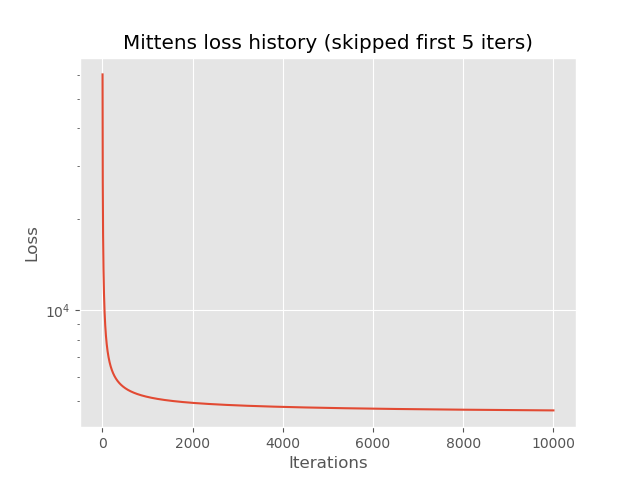
\includegraphics{exp_v2_loss.png} 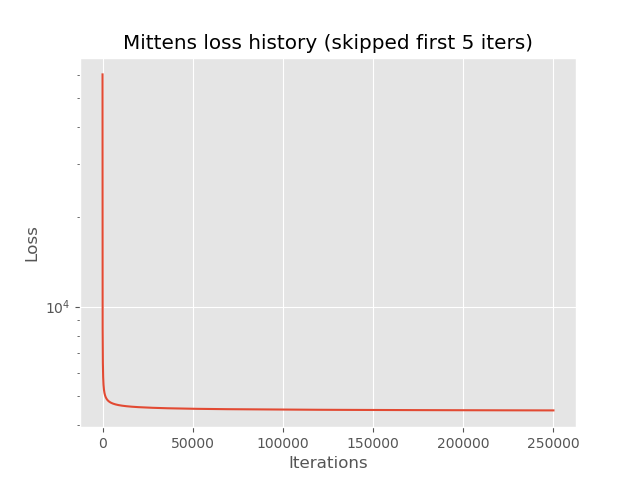
\includegraphics{exp_v1_loss.png}

We compare the resulting embeddings based on our neighborhood similarity
tests.

\emph{A secondary class entitled \texttt{EmbedsEngine} has been
developed. It encapsulates methods for post-processing, visualization
and high-end features based on pre-trained ProVe models}

		\begin{Verbatim}[commandchars=\\\{\},fontsize=\scriptsize]
{\color{incolor}In [{\color{incolor}15}]:} \PY{n}{prove\PYZus{}model} \PY{o}{=} \PY{n}{ProVe}\PY{p}{(}
             \PY{n}{default\PYZus{}embeds\PYZus{}file}\PY{o}{=}\PY{n}{EMB128\PYZus{}250k}\PY{p}{,}
             \PY{n}{name}\PY{o}{=}\PY{l+s+s1}{\PYZsq{}}\PY{l+s+s1}{exp\PYZus{}v1}\PY{l+s+s1}{\PYZsq{}}\PY{p}{,}
             \PY{n}{log}\PY{o}{=}\PY{n}{log}\PY{p}{,}
             \PY{p}{)}
         
         \PY{k}{if} \PY{n}{prove\PYZus{}model}\PY{o}{.}\PY{n}{embeds} \PY{o+ow}{is} \PY{k+kc}{None}\PY{p}{:}
             \PY{n}{prove\PYZus{}model}\PY{o}{.}\PY{n}{fit}\PY{p}{(}
                 \PY{n}{mco}\PY{o}{=}\PY{n}{csr\PYZus{}mco}\PY{p}{,}
                 \PY{n}{embed\PYZus{}size}\PY{o}{=}\PY{n}{EMBED\PYZus{}SIZE}\PY{p}{,}
                 \PY{n}{max\PYZus{}cooccure}\PY{o}{=}\PY{n}{MAX\PYZus{}FREQ}\PY{p}{,}
                 \PY{n}{epochs}\PY{o}{=}\PY{n}{MAX\PYZus{}ITERS}\PY{p}{,}
                 \PY{n}{save\PYZus{}folder}\PY{o}{=}\PY{n}{MODEL\PYZus{}HOME}\PY{p}{,}
                 \PY{n}{save\PYZus{}iters}\PY{o}{=}\PY{n}{SAVE\PYZus{}ITERS}\PY{p}{,}
             \PY{p}{)}
         
         \PY{n}{embeds} \PY{o}{=} \PY{n}{prove\PYZus{}model}\PY{o}{.}\PY{n}{embeds}
         
         \PY{n}{prod\PYZus{}eng} \PY{o}{=} \PY{n}{EmbedsEngine}\PY{p}{(}
             \PY{n}{np\PYZus{}embeddings}\PY{o}{=}\PY{n}{embeds}\PY{p}{,}
             \PY{n}{df\PYZus{}metadata}\PY{o}{=}\PY{n}{df\PYZus{}meta}\PY{p}{,}
             \PY{n}{name\PYZus{}field}\PY{o}{=}\PY{l+s+s1}{\PYZsq{}}\PY{l+s+s1}{ItemName}\PY{l+s+s1}{\PYZsq{}}\PY{p}{,}
             \PY{n}{id\PYZus{}field}\PY{o}{=}\PY{l+s+s1}{\PYZsq{}}\PY{l+s+s1}{IDE}\PY{l+s+s1}{\PYZsq{}}\PY{p}{,}
             \PY{n}{log}\PY{o}{=}\PY{n}{log}\PY{p}{,}
             \PY{n}{categ\PYZus{}fields}\PY{o}{=}\PY{p}{[}\PY{l+s+s1}{\PYZsq{}}\PY{l+s+s1}{Ierarhie1}\PY{l+s+s1}{\PYZsq{}}\PY{p}{,} \PY{l+s+s1}{\PYZsq{}}\PY{l+s+s1}{Ierarhie2}\PY{l+s+s1}{\PYZsq{}}\PY{p}{]}\PY{p}{,}
             \PY{n}{dct\PYZus{}categ\PYZus{}names}\PY{o}{=}\PY{n}{dct\PYZus{}categories}
             \PY{p}{)}
\end{Verbatim}

\begin{Verbatim}[commandchars=\\\{\},fontsize=\footnotesize]
ProVe embeds (13000, 128) loaded.
Found category string in 'Ierarhie1\_name'
Found category string in 'Ierarhie2\_name'
Constructing items knowledge graph
  Retrieving products for category 'Ierarhie1'
  Retrieving products for category 'Ierarhie2'
  Created products graph 100.0\%

\end{Verbatim}

    \hypertarget{refining-evaluation-data-using-trained-prove}{%
\subsection{Refining evaluation data using trained
ProVe}\label{refining-evaluation-data-using-trained-prove}}

Following the full generation of the ProVe vector space model for
product embeddings we can run few neighbors tests of our items expecting
similar results as with the word embeddings. As previously mentioned we
selected manually each individual evaluation item in order to find those
that would clearly fail at proposing a good replacement candidate with
just a cosine distance neighbor search within the products vector space.

Aside from the straightforward neighborhood search we also hand-picked
two other products - one that is obviously a potential replacement for
our product (``Best of David Bowie - 2002'') and another one that is
clearly not a replacement (``NLP - by Ian McDermott''). For these two
additional products we constantly measure the distances during the
various phases of our experiment.

		\begin{Verbatim}[commandchars=\\\{\},fontsize=\scriptsize]
{\color{incolor}In [{\color{incolor}16}]:} \PY{n}{test\PYZus{}items} \PY{o}{=} \PY{p}{[}
             \PY{l+m+mi}{12071}\PY{p}{,} \PY{l+m+mi}{11418}\PY{p}{,} \PY{l+m+mi}{10088}\PY{p}{,} \PY{l+m+mi}{9251}\PY{p}{,}
             \PY{l+m+mi}{9845}\PY{p}{,} \PY{l+m+mi}{8956}\PY{p}{,} \PY{l+m+mi}{6020}\PY{p}{,}
             \PY{l+m+mi}{129}\PY{p}{,} \PY{l+m+mi}{1150}\PY{p}{,} \PY{l+m+mi}{3852}
         \PY{p}{]}
         \PY{n}{exp\PYZus{}id} \PY{o}{=} \PY{l+m+mi}{12071}
         \PY{n}{pos\PYZus{}id} \PY{o}{=} \PY{l+m+mi}{11418}
         \PY{n}{neg\PYZus{}id} \PY{o}{=} \PY{l+m+mi}{5312}
         
         \PY{n}{prod\PYZus{}eng}\PY{o}{.}\PY{n}{analize\PYZus{}item}\PY{p}{(}\PY{n}{exp\PYZus{}id}\PY{p}{,} \PY{n}{positive\PYZus{}id}\PY{o}{=}\PY{n}{pos\PYZus{}id}\PY{p}{,} \PY{n}{negative\PYZus{}id}\PY{o}{=}\PY{n}{neg\PYZus{}id}\PY{p}{)}
         \PY{n}{prod\PYZus{}eng}\PY{o}{.}\PY{n}{get\PYZus{}similar\PYZus{}items}\PY{p}{(}\PY{n}{exp\PYZus{}id}\PY{p}{,} \PY{n}{filtered}\PY{o}{=}\PY{k+kc}{False}\PY{p}{,} \PY{n}{show}\PY{o}{=}\PY{n}{print\PYZus{}df}\PY{p}{)}
\end{Verbatim}

\begin{Verbatim}[commandchars=\\\{\},fontsize=\footnotesize]
Analysis of 12071: 'CD / DAVID BOWIE / BLACKSTAR (2016)'
  Distance from positive 11418:  0.921
  Distance from negative 5312:   0.653

\end{Verbatim}



    \begin{center}
\scriptsize
\begin{tabular}{lrrlll}
\toprule
{} &     ID &    DIST &                                      NAME &               H1 &                    H2 \\
\midrule
\textbf{0} &  12071 &  0.0000 &       CD / DAVID BOWIE / BLACKSTAR (2016) &           MUZICA &      CD International \\
\textbf{1} &   5312 &  0.6531 &  IAN MCDERMOTT / NLP PENTRU CARIERA SI VI &        CARTE ROM &  DEZVOLTARE PERSONALA \\
\textbf{2} &   9997 &  0.6543 &                    HOLLY SMALE / TOCILARA &        CARTE ROM &  FICTIUNE ADOLESCENTI \\
\textbf{3} &   1115 &  0.6829 &  DAN LUNGU / SUNT O BABA COMUNISTA (TOP10 &        CARTE ROM &              FICTIUNE \\
\textbf{4} &  10047 &  0.6899 &             MAGNET METAL - BATMAN (JOKER) &     COMICS\&MANGA &                Comics \\
\textbf{5} &   2883 &  0.6930 &  HARRIET MUNCASTER / ISADORA MOON MERGE C &        CARTE ROM &    CARTI PENTRU COPII \\
\textbf{6} &  12399 &  0.7012 &  YOU GIVE ME A REASON MINI CARD / KELLY H &     PAPETARIE AA &               Cadouri \\
\textbf{7} &   7132 &  0.7027 &  SALLY GARDNER / ARIPI SI CO 3: MISTERIOA &        CARTE ROM &    CARTI PENTRU COPII \\
\textbf{8} &   6443 &  0.7119 &                      DVD / DUNKIRK (2017) &       MULTIMEDIA &                   DVD \\
\textbf{9} &   9334 &  0.7229 &            SET 6 COASTERS PARIS MONUMENTS &  ACCESORII GASTR &  Accesorii servit mas \\
\bottomrule
\end{tabular}
\end{center}


    


    As we can see from above table our proposed ``anchor'' product
(\texttt{12071}) is clearly \emph{closer} to a lot of products that
might be in a complementarity relationship to it than to products from
its own category (music, rock, etc). We can run the same similarity
analysis using a filter that would give us only products from the same
generic inventory hierarchical category.

		\begin{Verbatim}[commandchars=\\\{\},fontsize=\scriptsize]
{\color{incolor}In [{\color{incolor}17}]:} \PY{n}{prod\PYZus{}eng}\PY{o}{.}\PY{n}{get\PYZus{}similar\PYZus{}items}\PY{p}{(}\PY{l+m+mi}{12071}\PY{p}{,} \PY{n}{filtered}\PY{o}{=}\PY{k+kc}{True}\PY{p}{,} \PY{n}{show}\PY{o}{=}\PY{n}{print\PYZus{}df}\PY{p}{)}
\end{Verbatim}



    \begin{center}
\scriptsize
\begin{tabular}{lrrlll}
\toprule
{} &     ID &    DIST &                                      NAME &      H1 &                   H2 \\
\midrule
\textbf{0  } &  12071 &  0.0000 &       CD / DAVID BOWIE / BLACKSTAR (2016) &  MUZICA &     CD International \\
\textbf{140} &  10604 &  0.7962 &  LP / LED ZEPPELIN / PHYSICAL GRAFFITI -1 &  MUZICA &                Vinyl \\
\textbf{205} &   9991 &  0.8102 &  CD / LED ZEPPELIN / REMASTERS (1990) CD2 &  MUZICA &     CD International \\
\textbf{219} &   8599 &  0.8127 &  CD / AC/DC / BACK IN BLACK -1980- (2003) &  MUZICA &     CD International \\
\textbf{453} &   3139 &  0.8368 &  CD / METALLICA / MASTER OF PUPPETS (1986 &  MUZICA &     CD International \\
\textbf{515} &   9333 &  0.8414 &    CD / GREEN DAY / AMERICAN IDIOT (2004) &  MUZICA &     CD International \\
\textbf{638} &   9811 &  0.8509 &  LP / ELVIS PRESLEY / THE ESSENTIAL (2016 &  MUZICA &                Vinyl \\
\textbf{677} &   7932 &  0.8533 &         CD / METALLICA / METALLICA (1991) &  MUZICA &     CD International \\
\textbf{690} &   6256 &  0.8541 &  LP / RED HOT CHILI PEPPERS / CALIFORNICA &  MUZICA &                Vinyl \\
\textbf{710} &   7645 &  0.8552 &       CD / DELIA / LIVE (DIGIPACK) (2017) &  MUZICA &  CD Repertoriu Local \\
\bottomrule
\end{tabular}
\end{center}


    


    We also test the embeddings resulted from the 10,000 epochs training.
Worth to mention is that the GPU 10,000 iterations took around 40' while
the 250,000 took more than 12 hours. We discover that the lower epochs
model behaves radically better than the 12 hrs trained model pointing to
further investigation and the implementation of additional optimization
heuristics (such as an early stopping mechanism)

		\begin{Verbatim}[commandchars=\\\{\},fontsize=\scriptsize]
{\color{incolor}In [{\color{incolor}30}]:} \PY{n}{embeds\PYZus{}10ke} \PY{o}{=} \PY{n}{np}\PY{o}{.}\PY{n}{load}\PY{p}{(}\PY{n}{EMB128\PYZus{}10k}\PY{p}{)}
         \PY{n}{prod\PYZus{}eng}\PY{o}{.}\PY{n}{analize\PYZus{}item}\PY{p}{(}\PY{n}{exp\PYZus{}id}\PY{p}{,} \PY{n}{positive\PYZus{}id}\PY{o}{=}\PY{n}{pos\PYZus{}id}\PY{p}{,} \PY{n}{negative\PYZus{}id}\PY{o}{=}\PY{n}{neg\PYZus{}id}\PY{p}{,}
         \PY{n}{embeds}\PY{o}{=}\PY{n}{embeds\PYZus{}10ke}\PY{p}{)}
         \PY{n}{prod\PYZus{}eng}\PY{o}{.}\PY{n}{get\PYZus{}similar\PYZus{}items}\PY{p}{(}\PY{n}{exp\PYZus{}id}\PY{p}{,} \PY{n}{filtered}\PY{o}{=}\PY{k+kc}{False}\PY{p}{,} \PY{n}{show}\PY{o}{=}\PY{n}{print\PYZus{}df}\PY{p}{,} \PY{n}{embeds}\PY{o}{=}\PY{n}{embeds\PYZus{}10ke}\PY{p}{)}
\end{Verbatim}

\begin{Verbatim}[commandchars=\\\{\},fontsize=\footnotesize]
Analysis of 12071: 'CD / DAVID BOWIE / BLACKSTAR (2016)'
  Distance from positive 11418:  0.664
  Distance from negative 5312:   1.010

\end{Verbatim}



    \begin{center}
\scriptsize
\begin{tabular}{lrrlll}
\toprule
{} &     ID &  DIST &                                      NAME &             H1 &                   H2 \\
\midrule
\textbf{0} &  12071 & 0.000 &       CD / DAVID BOWIE / BLACKSTAR (2016) &         MUZICA &     CD International \\
\textbf{1} &  11418 & 0.664 &  CD / DAVID BOWIE / BEST OF BOWIE (2002)  &         MUZICA &     CD International \\
\textbf{2} &  10035 & 0.688 &  CD / AEROSMITH / THE ESSENTIAL AEROSMITH &         MUZICA &     CD International \\
\textbf{3} &   9040 & 0.689 &  CD / LEONARD COHEN / YOU WANT IT DARKER  &         MUZICA &     CD International \\
\textbf{4} &   5707 & 0.691 &    PLASTILINA  AMOS 4/SET IC18P4 (B X 12) &        JUCARII &         Necatalogate \\
\textbf{5} &   8639 & 0.699 &  KNOCK KNOCK 100 REASON TO PANIC BOOK ABO &  CARTE STRAINA &           GIFT BOOKS \\
\textbf{6} &   1352 & 0.704 &  PLASTILINA  AMOS PVCIC18G 18G/CUTIE GALB &        JUCARII &         Necatalogate \\
\textbf{7} &   6964 & 0.708 &  CELLA SERGHI / PE FIRUL DE PAIANJEN AL M &      CARTE ROM &  BIOGRAFII / MEMORII \\
\textbf{8} &   8807 & 0.709 &          SIMON SEBAG MONTEFIORE / SASENKA &      CARTE ROM &             FICTIUNE \\
\textbf{9} &  12668 & 0.712 &   DAVID MCKEE / PRIMA MEA CARTICICA ELMER &      CARTE ROM &   CARTI PENTRU COPII \\
\bottomrule
\end{tabular}
\end{center}


    


    \hypertarget{the-full-pipeline}{%
\section{The full Pipeline}\label{the-full-pipeline}}

There are two main pipelines, one for each of our two individual
objectives : that of finding product replacements and the second one of
cold-start-ing new products in inventories:

\textbf{Algorithm \#1 \texttt{GetProductReplacement} - Product
Replacement Modelling pipeline}

\begin{verbatim}
 1. Create MCO
 2. Apply ProVe and obtain item embeddings
 3. Extract knowledge graph information from meta-data  
 4. For each individual product  
     4.1. Find connected products  
     4.2. Retrofit the product using connected products  
\end{verbatim}

\textbf{Algorithm \#2 \texttt{ColdStartProduct} - cold-starting new
products embeddings}

\begin{verbatim}
 1. Setup embeddings of existing products and extract knowledge graph information from meta-data
 2. Input new product hierarchy information
 3. Input similar products from proposed similar products
 4. Create new product embedding based on proposed similar with simple mean over embeddings
 5. Add all hierarchy-based products to the list of similar products
 6. Retrofit the new product embedding to all similar products 
\end{verbatim}

At this point we have discussed regarding the MCO preparation and
processing the count matrix with \emph{ProVe} in order to obtain the
initial products embedding space. The next logical step (\texttt{2.} in
our algorithm) is to process the available hierarchical information in
order to construct the knowledge graph. For this we are going to treat
each category provided by the inventory's category management database
as a potential source of information that can provide knowledge graph
edges for each product in its domain. For our previous item example
\texttt{12071} (David Bowie's ``Blackstar'') the product information is
presented below:

		\begin{Verbatim}[commandchars=\\\{\},fontsize=\scriptsize]
{\color{incolor}In [{\color{incolor}18}]:} \PY{n}{dct\PYZus{}prod\PYZus{}info} \PY{o}{=} \PY{n}{prod\PYZus{}eng}\PY{o}{.}\PY{n}{get\PYZus{}item\PYZus{}info}\PY{p}{(}\PY{n}{exp\PYZus{}id}\PY{p}{,} \PY{n}{verbose}\PY{o}{=}\PY{k+kc}{True}\PY{p}{)}
\end{Verbatim}

\begin{Verbatim}[commandchars=\\\{\},fontsize=\footnotesize]
Product '12071' info:
  NAME: CD / DAVID BOWIE / BLACKSTAR (2016)
  Level 'Ierarhie1': 2
  Level 'Ierarhie1\_name': MUZICA
  Level 'Ierarhie2': 4
  Level 'Ierarhie2\_name': CD International
  EDGES: \{10759, 1032, 12305, 3091, 4627, 10780, 9251, 1232

\end{Verbatim}

    At this point we can proceed with the final step presented in Algorithm
\#1, that of using the knowledge graph and pulling closer the products
that have edges. Our proposed framework has multiple flavors when it
comes to selecting the part of the embedding space we want to modify and
in this case, for the sake of the experiment and for a clearer
intuition, we chose only to modify the vector space portion that is most
relevant for our chose product (\texttt{12071})

		\begin{Verbatim}[commandchars=\\\{\},fontsize=\scriptsize]
{\color{incolor}In [{\color{incolor}19}]:} \PY{n}{new\PYZus{}embeds} \PY{o}{=} \PY{n}{prod\PYZus{}eng}\PY{o}{.}\PY{n}{get\PYZus{}retrofitted\PYZus{}embeds}\PY{p}{(}\PY{n}{prod\PYZus{}ids}\PY{o}{=}\PY{n}{exp\PYZus{}id}\PY{p}{,} \PY{n}{method}\PY{o}{=}\PY{l+s+s1}{\PYZsq{}}\PY{l+s+s1}{v1}\PY{l+s+s1}{\PYZsq{}}\PY{p}{)}
\end{Verbatim}

\begin{Verbatim}[commandchars=\\\{\},fontsize=\footnotesize]
Performing retrofitting on (13000, 128) embedding matrix{\ldots}
  Stop tel:    5.0e-03
  Start-edges: 1
Iteration 1; change was 3.5e+00
Iteration 2; change was 8.0e-03
Retrofiting converged at iteration 3; change was 0.0000

\end{Verbatim}

    The next logical step is to verify the results of our retrofitting
process re-running the past neighborhood tests both with and without
filtering. First we run the search with no filtering:

		\begin{Verbatim}[commandchars=\\\{\},fontsize=\scriptsize]
{\color{incolor}In [{\color{incolor}20}]:} \PY{n}{prod\PYZus{}eng}\PY{o}{.}\PY{n}{get\PYZus{}similar\PYZus{}items}\PY{p}{(}\PY{n}{exp\PYZus{}id}\PY{p}{,} \PY{n}{embeds}\PY{o}{=}\PY{n}{new\PYZus{}embeds}\PY{p}{,} \PY{n}{filtered}\PY{o}{=}\PY{k+kc}{False}\PY{p}{,} \PY{n}{show}\PY{o}{=}\PY{n}{print\PYZus{}df}\PY{p}{)}
\end{Verbatim}



    \begin{center}
\scriptsize
\begin{tabular}{lrrlll}
\toprule
{} &     ID &        DIST &                                      NAME &               H1 &                    H2 \\
\midrule
\textbf{0} &  12071 &  1.7881e-07 &       CD / DAVID BOWIE / BLACKSTAR (2016) &           MUZICA &      CD International \\
\textbf{1} &   5312 &  6.6791e-01 &  IAN MCDERMOTT / NLP PENTRU CARIERA SI VI &        CARTE ROM &  DEZVOLTARE PERSONALA \\
\textbf{2} &   9997 &  6.7252e-01 &                    HOLLY SMALE / TOCILARA &        CARTE ROM &  FICTIUNE ADOLESCENTI \\
\textbf{3} &  10047 &  6.8937e-01 &             MAGNET METAL - BATMAN (JOKER) &     COMICS\&MANGA &                Comics \\
\textbf{4} &   1115 &  6.9019e-01 &  DAN LUNGU / SUNT O BABA COMUNISTA (TOP10 &        CARTE ROM &              FICTIUNE \\
\textbf{5} &   7132 &  6.9034e-01 &  SALLY GARDNER / ARIPI SI CO 3: MISTERIOA &        CARTE ROM &    CARTI PENTRU COPII \\
\textbf{6} &   6443 &  6.9186e-01 &                      DVD / DUNKIRK (2017) &       MULTIMEDIA &                   DVD \\
\textbf{7} &  12399 &  7.0380e-01 &  YOU GIVE ME A REASON MINI CARD / KELLY H &     PAPETARIE AA &               Cadouri \\
\textbf{8} &   2883 &  7.0732e-01 &  HARRIET MUNCASTER / ISADORA MOON MERGE C &        CARTE ROM &    CARTI PENTRU COPII \\
\textbf{9} &   9334 &  7.2087e-01 &            SET 6 COASTERS PARIS MONUMENTS &  ACCESORII GASTR &  Accesorii servit mas \\
\bottomrule
\end{tabular}
\end{center}


    


    And then we run it with filtering using the hierarchy management
database.

		\begin{Verbatim}[commandchars=\\\{\},fontsize=\scriptsize]
{\color{incolor}In [{\color{incolor}21}]:} \PY{n}{df} \PY{o}{=} \PY{n}{prod\PYZus{}eng}\PY{o}{.}\PY{n}{get\PYZus{}similar\PYZus{}items}\PY{p}{(}\PY{n}{exp\PYZus{}id}\PY{p}{,} \PY{n}{embeds}\PY{o}{=}\PY{n}{new\PYZus{}embeds}\PY{p}{,} \PY{n}{filtered}\PY{o}{=}\PY{k+kc}{True}\PY{p}{,} \PY{n}{show}\PY{o}{=}\PY{n}{print\PYZus{}df}\PY{p}{)}
\end{Verbatim}

    Now we can repeat our hand-picked positive vs negative examples test and
observe an improvement in the distances (slightly lower for the positive
and slightly higher for the negative). However, this improvement is far
from our desired objective of determining the replacement (the actual
positive example in this case) with the simple cosine distance
measurement.

		\begin{Verbatim}[commandchars=\\\{\},fontsize=\scriptsize]
{\color{incolor}In [{\color{incolor}22}]:} \PY{n}{prod\PYZus{}eng}\PY{o}{.}\PY{n}{analize\PYZus{}item}\PY{p}{(}\PY{n}{exp\PYZus{}id}\PY{p}{,} \PY{n}{positive\PYZus{}id}\PY{o}{=}\PY{n}{pos\PYZus{}id}\PY{p}{,} \PY{n}{negative\PYZus{}id}\PY{o}{=}\PY{n}{neg\PYZus{}id}\PY{p}{,} \PY{n}{embeds}\PY{o}{=}\PY{n}{new\PYZus{}embeds}\PY{p}{)}
\end{Verbatim}

\begin{Verbatim}[commandchars=\\\{\},fontsize=\footnotesize]
Analysis of 12071: 'CD / DAVID BOWIE / BLACKSTAR (2016)'
  Distance from positive 11418:  0.903
  Distance from negative 5312:   0.668

\end{Verbatim}

    \hypertarget{progress-history}{%
\section{Progress history}\label{progress-history}}

At this point in our research and development process we managed to
obtain generate the product embeddings based starting from the real-life
transactional database. A more important finding is that we have
experimental proof that our \emph{ProVe} model shows clear signs of
capturing ``semantic'' information regarding product similarities as
well as product complementarity, albeit without a clear cut between the
two distinct categories. Similar findings can be discerned from the
early work of Grbovic et al \cite{grbovic2015commerce} who use the
k-means based clusters in order to separate potential similarities from
complementarities.

Progress has also been made with regard to the final stages of the
proposed pipeline as the first iteration of experimentation with Faruqui
et al \cite{faruqui2014retrofitting} has been implemented as presented
before.

There is still a extensive list of actions and problems that have to be
tackled such as:

\begin{enumerate}
\def\labelenumi{\arabic{enumi}.}
\tightlist
\item
  Review the ProVe training and find the required heuristics that would
  aid us in finind the best time-vs-embeddings quality ratio.
\item
  Review the knowledge graph preparation process as well as optimize the
  v1 retrofitting method
\item
  Tune the ProVe hyperparameters and scalability. Re-train the model
  with maximum energy efficiency vs performance
\item
  Evaluate these initial results with the proposed \texttt{MRR} metric
  on a larger set of manually chosen items
\item
  Add optimized versions of the retrofitting as well as functional
  retrofitting (Lengerich et al \cite{lengerich2017retrofitting})
\item
  Evaluate the results for the advanced methods and compare with (1)
\item
  Complete the \texttt{ColdStartProduct} pipeline (Algorithm \#2)
\end{enumerate}

		\begin{Verbatim}[commandchars=\\\{\},fontsize=\scriptsize]
{\color{incolor}In [{\color{incolor}23}]:} \PY{n}{printmd}\PY{p}{(}\PY{l+s+s2}{\PYZdq{}}\PY{l+s+s2}{END of Experimental Protocol.}\PY{l+s+s2}{\PYZdq{}}\PY{p}{)}
\end{Verbatim}


    END of Experimental Protocol.

    


    % Add a bibliography block to the postdoc
    
    
\bibliographystyle{unsrt}
\bibliography{jupyter}

    
\end{document}
